\documentclass[12pt, openany, oneside]{book}

\usepackage{listings}
\usepackage[dvipsnames]{xcolor}
\usepackage{ctex}
\usepackage{fontspec}
\usepackage{setspace}
\usepackage{tikz}
\usepackage{anyfontsize}
\usepackage{sectsty}
\usepackage{titlesec}
\usepackage{float}
\usepackage[hidelinks]{hyperref}
\usepackage[a4paper]{geometry}
\usepackage{url}
\usepackage{amssymb}
\usepackage{fontawesome5}
\usepackage[most]{tcolorbox}
\usepackage{circuitikz}
\usepackage{stackengine}
% \usepackage{minted}

\usetikzlibrary{calc,trees,positioning,arrows,fit,shapes,calc}
\usetikzlibrary{calc}
\usetikzlibrary{calc,shapes.multipart,chains,arrows}

\def\rlwd{.5pt} \def\rlht{2.2ex} \def\rldp{.5ex}
\def\mydiv#1{~%
  \rule[-\rldp]{\rlwd}{\rlht}%
  \setbox0=\hbox{~#1}%
  \stackunder[\dimexpr\rldp-\rlwd]{~#1}{\rule{\wd0}{\rlwd}}%
}

\definecolor{mycolor}{RGB}{0,128,128}
\newtcbox{\mybox} {
    on line,
    colback=mycolor,
    fontupper=\bfseries\color{white},
    boxrule=0pt,
    arc=5pt, 
    boxsep=0pt, 
    left=2pt, 
    right=2pt, 
    top=5pt, 
    bottom=5pt
}

\setstretch{1.5}
\setlength{\parindent}{0cm}

\geometry{a4paper,top=2.5cm,bottom=2.5cm}

\titleformat{\chapter}{\Huge\Huge\bfseries}{\chaptertitlename\ \thechapter{\ }}{0pt}{\Huge}{}
\titlespacing{\chapter}{0pt}{0pt}{12pt}

\definecolor{dkgreen}{rgb}{0,0.4,0}
\definecolor{gray}{rgb}{0.5,0.5,0.5}
\definecolor{mauve}{rgb}{0.58,0,0.82}
\definecolor{LightGray}{gray}{0.9}

\lstset{
    basicstyle=\normalsize \fontspec{Consolas},    %  the size of the fonts that are used for the code
    numbers=left,            % where to put the line-numbers
    numberstyle=\color{black},  % the style that is used for the line-numbers
    numbersep=10pt,                  % how far the line-numbers are from the code
    backgroundcolor=\color{white},
    showspaces=false,
    showstringspaces=false,
    showtabs=false,
    frame=single,                   % adds a frame around the code
    rulecolor=\color{black},        % if not set, the frame-color may be changed on line-breaks within not-black text (e.g. commens (green here))
    tabsize=4,                      % sets default tabsize to 2 spaces
    captionpos=t,                   % sets the caption-position to bottom
    breaklines=false,                % sets automatic line breaking
    breakatwhitespace=true,        % sets if automatic breaks should only happen at whitespace
    title=\lstname,                   % show the filename of files included with \lstinputlisting;
    % also try caption instead of title
    numberstyle=\color{black},		% line number color
    keywordstyle=\color{blue},          % keyword style
    commentstyle=\color{dkgreen},       % comment style
    stringstyle=\color{mauve},         % string literal style
    escapeinside={\%*}{*)},            % if you want to add LaTeX within your code
    morekeywords={*,...}               % if you want to add more keywords to the set
}

\begin{document}

\pagestyle{plain}

\begin{tikzpicture}[overlay,remember picture]
	% Background color
	\fill[
		black!2]
	(current page.south west) rectangle (current page.north east);

	% Rectangles
	\shade[
		left color=Dandelion,
		right color=Dandelion!40,
		transform canvas ={rotate around ={45:($(current page.north west)+(0,-6)$)}}]
	($(current page.north west)+(0,-6)$) rectangle ++(9,1.5);

	\shade[
		left color=lightgray,
		right color=lightgray!50,
		rounded corners=0.75cm,
		transform canvas ={rotate around ={45:($(current page.north west)+(.5,-10)$)}}]
	($(current page.north west)+(0.5,-10)$) rectangle ++(15,1.5);

	\shade[
		left color=lightgray,
		rounded corners=0.3cm,
		transform canvas ={rotate around ={45:($(current page.north west)+(.5,-10)$)}}] ($(current page.north west)+(1.5,-9.55)$) rectangle ++(7,.6);

	\shade[
		left color=orange!80,
		right color=orange!60,
		rounded corners=0.4cm,
		transform canvas ={rotate around ={45:($(current page.north)+(-1.5,-3)$)}}]
	($(current page.north)+(-1.5,-3)$) rectangle ++(9,0.8);

	\shade[
		left color=red!80,
		right color=red!80,
		rounded corners=0.9cm,
		transform canvas ={rotate around ={45:($(current page.north)+(-3,-8)$)}}] ($(current page.north)+(-3,-8)$) rectangle ++(15,1.8);

	\shade[
		left color=orange,
		right color=Dandelion,
		rounded corners=0.9cm,
		transform canvas ={rotate around ={45:($(current page.north west)+(4,-15.5)$)}}]
	($(current page.north west)+(4,-15.5)$) rectangle ++(30,1.8);

	\shade[
		left color=RoyalBlue,
		right color=Emerald,
		rounded corners=0.75cm,
		transform canvas ={rotate around ={45:($(current page.north west)+(13,-10)$)}}]
	($(current page.north west)+(13,-10)$) rectangle ++(15,1.5);

	\shade[
		left color=lightgray,
		rounded corners=0.3cm,
		transform canvas ={rotate around ={45:($(current page.north west)+(18,-8)$)}}]
	($(current page.north west)+(18,-8)$) rectangle ++(15,0.6);

	\shade[
		left color=lightgray,
		rounded corners=0.4cm,
		transform canvas ={rotate around ={45:($(current page.north west)+(19,-5.65)$)}}]
	($(current page.north west)+(19,-5.65)$) rectangle ++(15,0.8);

	\shade[
		left color=OrangeRed,
		right color=red!80,
		rounded corners=0.6cm,
		transform canvas ={rotate around ={45:($(current page.north west)+(20,-9)$)}}]
	($(current page.north west)+(20,-9)$) rectangle ++(14,1.2);

	% Year
	% \draw[ultra thick,gray]
	% ($(current page.center)+(5,2)$) -- ++(0,-3cm)
	node[
			midway,
			left=0.25cm,
			text width=5cm,
			align=right,
			black!75
		]
		{
			% {\fontsize{25}{30} \selectfont \bf ANNUAL \\[10pt] REPORT}
		}
	node[
			midway,
			right=0.25cm,
			text width=6cm,
			align=left,
			orange]
		{
			% {\fontsize{72}{86.4} \selectfont 2020}
		};

	% Title
	\node[align=center] at ($(current page.center)+(0,-5)$)
	{
	{\fontsize{72}{72} \selectfont {{离散数学}}} \\[1cm]
	{\fontsize{42}{42} \selectfont {{Discrete Mathematics}}} \\[2cm]
	{\fontsize{20}{19.2} \selectfont \textcolor{orange}{ \bf 极夜酱}} \\[4pt]
	};
\end{tikzpicture}

\newpage

\setcounter{tocdepth}{1}
\tableofcontents
\thispagestyle{empty}

\newpage

\setcounter{page}{1}

\chapter{逻辑}

\section{命题}

\subsection{命题(Proposition)}

逻辑(logic)规则给出数学语句的准确含义,这些规则用来区分有效和无效的数学论证。逻辑不仅对理解数学推理十分重要,而且在计算机科学中有许多应用,逻辑可用于电路设计、程序构造、程序正确性证明等方面。 \\

命题是逻辑的基本成分,一个命题是一个具有真值(truth value)的语句,命题可以为真也可以为假,但不能既为真又为假。 \\

\begin{table}[H]
	\centering
	\setlength{\tabcolsep}{5mm}{
		\begin{tabular}{|c|c|}
			\hline
			\textbf{命题}        & \textbf{非命题}    \\
			\hline
			I have a dog.        & What day is today? \\
			\hline
			1 + 2 = 3            & Shut the door!     \\
			\hline
			Today is Wednesday.  & 1 + 2              \\
			\hline
			It is snowing today. & x + 1 = 2          \\
			\hline
		\end{tabular}
	}
\end{table}

命题习惯上用字母$ p $, $ q $, $ r $, $ s $等来表示,如果一个命题是真命题,它的真值为真,用T表示;如果一个命题是假命题,它的真值为假,用F表示。 \\

\subsection{非运算符(NOT, Negation Operator)}

非运算符$ \neg $只作用于一个命题,其作用是反转命题的真值。 \\

真值表(truth table)可以给出命题真值之间的关系,在确定由简单命题组成的命题的真值时,真值表特别有用。

\begin{table}[H]
	\centering
	\setlength{\tabcolsep}{5mm}{
		\begin{tabular}{|c|c|}
			\hline
			\textbf{$ p $} & \textbf{$ \neg p $} \\
			\hline
			T              & F                   \\
			\hline
			F              & T                   \\
			\hline
		\end{tabular}
	}
	\caption{NOT真值表}
\end{table}

\begin{tcolorbox}
	\mybox{Exercise}
	$ \neg p $ \\
	$ p $: It snowed last night. \\
	$ \neg p $: It didn;t snow last night. \\
	$ q $: $ 2 + 3 = 6 $ \\
	$ \neg q $: $ 2 + 3 \ne 6 $
\end{tcolorbox}

\subsection{合取运算符(AND, Conjunction Operator)}

命题$ p \wedge q $表示$ p $并且$ q $,当$ p $和$ q $都为真时命题为真,否则为假。

\begin{table}[H]
	\centering
	\setlength{\tabcolsep}{5mm}{
		\begin{tabular}{|c|c|c|}
			\hline
			\textbf{$ p $} & \textbf{$ \neg p $} & \textbf{$ p \wedge q $} \\
			\hline
			T              & T                   & T                       \\
			\hline
			T              & F                   & F                       \\
			\hline
			F              & T                   & F                       \\
			\hline
			F              & F                   & F                       \\
			\hline
		\end{tabular}
	}
	\caption{AND真值表}
\end{table}

\begin{tcolorbox}
	\mybox{Exercise}
	$ p \wedge q $ \\
	$ p $: 今天是星期五。 \\
	$ q $: 今天会下雨。 \\
	$ p \wedge q $: 今天是星期五并且会下雨。
\end{tcolorbox}

\subsection{析取运算符(OR, Disjunction Operator)}

命题$ p \vee q $表示$ p $或$ q $,当$ p $和$ q $都为假时命题为假,否则为真。

\begin{table}[H]
	\centering
	\setlength{\tabcolsep}{5mm}{
		\begin{tabular}{|c|c|c|}
			\hline
			\textbf{$ p $} & \textbf{$ \neg p $} & \textbf{$ p \vee q $} \\
			\hline
			T              & T                   & T                     \\
			\hline
			T              & F                   & T                     \\
			\hline
			F              & T                   & T                     \\
			\hline
			F              & F                   & F                     \\
			\hline
		\end{tabular}
	}
	\caption{OR真值表}
\end{table}

\begin{tcolorbox}
	\mybox{Exercise}
	$ p \vee q $ \\
	$ p $: 开关坏了。 \\
	$ q $: 灯泡坏了。 \\
	$ p \vee q $: 开关坏了或者灯泡坏了。
\end{tcolorbox}

\subsection{异或运算符(XOR, Exclusive Or)}

命题$ p \oplus q $表示$ p $和$ q $的异或,当$ p $和$ q $中恰有一个为真时命题为真,否则为假。

\begin{table}[H]
	\centering
	\setlength{\tabcolsep}{5mm}{
		\begin{tabular}{|c|c|c|}
			\hline
			\textbf{$ p $} & \textbf{$ \neg p $} & \textbf{$ p \oplus q $} \\
			\hline
			T              & T                   & F                       \\
			\hline
			T              & F                   & T                       \\
			\hline
			F              & T                   & T                       \\
			\hline
			F              & F                   & F                       \\
			\hline
		\end{tabular}
	}
	\caption{XOR真值表}
\end{table}

\begin{tcolorbox}
	\mybox{Exercise}
	$ p \oplus q $ \\
	$ p $: 他现在在上海。 \\
	$ q $: 他现在在北京。 \\
	$ p \vee q $: 他现在在上海或北京。
\end{tcolorbox}

\begin{tcolorbox}
	\mybox{Exercise}
	某地发生了一件谋杀案,警察通过排查确定杀人凶手必为4个嫌疑犯的一个,根据以下信息确定凶手。 \\
	A说:不是我。 \\
	B说:是C。 \\
	C说:是D。 \\
	D说:C在胡说。 \\
	已知3个人说了真话,1个人说的是假话。
\end{tcolorbox}

\begin{lstlisting}[language=Python]
def main():
    for killer in ['A', 'B', 'C', 'D']:
        if (killer != 'A') + (killer == 'C') \
            + (killer == 'D') + (killer != 'D') == 3:
            print(killer)

if __name__ == "__main__":
    main()
\end{lstlisting}

\begin{tcolorbox}
	\mybox{运行结果}
	C
\end{tcolorbox}

\newpage

\section{复合命题}

\subsection{复合命题(Compound Proposition)}

使用非运算符和已定义的各联结词可以构造复合命题。小括号用于规定复合命题中多个逻辑运算符的操作顺序,为了减少所需的小括号数量,规定了各联结词的优先级。

\begin{table}[H]
	\centering
	\setlength{\tabcolsep}{5mm}{
		\begin{tabular}{|c|c|}
			\hline
			\textbf{优先级} & \textbf{运算符}                   \\
			\hline
			1               & $ \neg $                          \\
			\hline
			2               & $ \wedge $ / $ \vee $             \\
			\hline
			3               & $ \rightarrow / \leftrightarrow $ \\
			\hline
		\end{tabular}
	}
	\caption{运算符优先级}
\end{table}

\subsection{蕴含运算符(Implication Operator)}

命题$ p \rightarrow q $表示$ p $蕴含$ q $,在$ p $为真而$ q $为假时命题为假,否则为真。其中$ p $称为前提,$ q $称为结论。

\begin{table}[H]
	\centering
	\setlength{\tabcolsep}{5mm}{
		\begin{tabular}{|c|c|c|}
			\hline
			\textbf{$ p $} & \textbf{$ q $} & \textbf{$ p \rightarrow q $} \\
			\hline
			T              & T              & T                            \\
			\hline
			T              & F              & F                            \\
			\hline
			F              & T              & T                            \\
			\hline
			F              & F              & T                            \\
			\hline
		\end{tabular}
	}
	\caption{蕴含真值表}
\end{table}

表示$ p \rightarrow q $的术语有很多种,常见的有:

\begin{itemize}
	\item If $ p $, then $ q $.
	\item $ p $ only if $ q $.
	\item $ q $ is necessary for $ p $.
\end{itemize}

\begin{tcolorbox}
	\mybox{Exercise}
	$ p \rightarrow q $ \\
	$ p $:我去看电影。 \\
	$ q $:我买奶茶。 \\
	$ p \rightarrow q $:如果我去看电影,那么我会买奶茶。
\end{tcolorbox}

\begin{figure}[H]
	\centering
	
\includegraphics[scale=0.7]{img/C1/1-2/1.png}
\end{figure}

由$ p \rightarrow q $可以构造出几个相关的蕴含:

\begin{enumerate}
	\item $ q \rightarrow p $称为$ p \rightarrow q $的逆命题(converse)。
	\item $ \neg q \rightarrow \neg p $称为$ p \rightarrow q $的逆否命题(contrapositive)。
\end{enumerate}

\begin{tcolorbox}
	\mybox{Exercise}
	逆命题与逆否命题 \\
	$ p $:今天是星期四。 \\
	$ q $:我今天有考试。 \\
	$ p \rightarrow q $:如果今天是星期四,那么我今天有考试。 \\
	$ q \rightarrow p $:如果我今天有考试,那么果今天是星期四。 \\
	$ \neg q \rightarrow \neg p $:如果我今天没有考试,那么今天不是星期四。
\end{tcolorbox}

\subsection{双向蕴含(Biconditional Operation)}

命题$ p \leftrightarrow q $表示$ p $双向蕴含$ q $,在$ p $和$ q $有相同的真值时命题为真,否则为假。

\begin{table}[H]
	\centering
	\setlength{\tabcolsep}{5mm}{
		\begin{tabular}{|c|c|c|}
			\hline
			\textbf{$ p $} & \textbf{$ q $} & \textbf{$ p \leftrightarrow q $} \\
			\hline
			T              & T              & T                                \\
			\hline
			T              & F              & F                                \\
			\hline
			F              & T              & F                                \\
			\hline
			F              & F              & T                                \\
			\hline
		\end{tabular}
	}
	\caption{双向蕴含真值表}
\end{table}

双蕴含的真值表与异或的真值表正好相反,因此$ p \leftrightarrow q $与$ \neg (p \oplus q) $等价。

\newpage

\section{逻辑等价}

\subsection{逻辑等价(Logical Equivalence)}

两个不同的复合命题可能拥有完全相同的真值,则称这两个命题在逻辑上是等价的。如果无论复合命题中各个命题的真值是什么,复合命题的真值总是为真,这样的复合命题称为永真式(tautology)。如果真值永远为假的复合命题称为矛盾(contradiction)。

\begin{table}[H]
	\centering
	\setlength{\tabcolsep}{5mm}{
		\begin{tabular}{|c|c|c|c|}
			\hline
			\textbf{$ p $} & \textbf{$ \neg p $} & \textbf{$ p \vee \neg p $} & \textbf{$ p \wedge \neg p $} \\
			\hline
			T              & F                   & T                          & F                            \\
			\hline
			F              & T                   & T                          & F                            \\
			\hline
		\end{tabular}
	}
	\caption{逻辑等价}
\end{table}

如果复合命题$ s $和是$ r $逻辑等价的,可表示为$ s \equiv r $。只有当$ s \leftrightarrow r $是永真式时,$ s $和$ r $才是逻辑等价的。

\begin{tcolorbox}
	\mybox{Exercise}
	使用真值表证明$ p \vee q \equiv \neg (\neg p \wedge \neg q) $
	\begin{table}[H]
		\centering
		\setlength{\tabcolsep}{5mm}{
			\begin{tabular}{|c|c|c|c|c|c|c|}
				\hline
				\textbf{$ p $} & \textbf{$ q $} & \textbf{$ p \vee q $} & \textbf{$ \neg p $} & \textbf{$ \neg q $} & \textbf{$ \neg p \wedge \neg q $} & \textbf{$ \neg (\neg p \wedge \neg q) $} \\
				\hline
				T              & T              & T                     & F                   & F                   & F                                 & T                                        \\
				\hline
				T              & F              & T                     & F                   & T                   & F                                 & T                                        \\
				\hline
				F              & T              & T                     & T                   & F                   & F                                 & T                                        \\
				\hline
				F              & F              & F                     & T                   & T                   & T                                 & F                                        \\
				\hline
			\end{tabular}
		}
	\end{table}
\end{tcolorbox}

\subsection{逻辑等价定理}

\begin{tcolorbox}
	\mybox{幂等律 Idempotent Laws}
	\begin{align}
		p \wedge p & \equiv p \\
		p \vee p   & \equiv p
	\end{align}
\end{tcolorbox}

\begin{tcolorbox}
	\mybox{恒等律 Identity Laws}
	\begin{align}
		p \wedge T & \equiv p \\
		p \vee F   & \equiv p
	\end{align}
\end{tcolorbox}

\begin{tcolorbox}
	\mybox{支配律 Domination Laws}
	\begin{align}
		p \vee T   & \equiv T \\
		p \wedge F & \equiv F
	\end{align}
\end{tcolorbox}

\begin{tcolorbox}
	\mybox{双非律 Double Negation Law}
	\begin{align}
		\neg (\neg p) & \equiv p
	\end{align}
\end{tcolorbox}

\begin{tcolorbox}
	\mybox{交换律 Commutative Laws}
	\begin{align}
		p \wedge q & \equiv q \wedge p \\
		p \vee q   & \equiv q \vee p
	\end{align}
\end{tcolorbox}

\begin{tcolorbox}
	\mybox{结合律 Associative Laws}
	\begin{align}
		(p \wedge q) \wedge r & \equiv p \wedge (q \wedge r) \\
		(p \vee q) \vee r     & \equiv p \vee (q \vee r)
	\end{align}
\end{tcolorbox}

\begin{tcolorbox}
	\mybox{分配律 Distributive Laws}
	\begin{align}
		(p \wedge q) \wedge r & \equiv p \wedge (q \wedge r) \\
		(p \vee q) \vee r     & \equiv p \vee (q \vee r)
	\end{align}
\end{tcolorbox}

\begin{tcolorbox}
	\mybox{德摩根律 De Morgan's Laws}
	\begin{align}
		\neg (p \wedge q) & \equiv \neg p \vee \neg q   \\
		\neg (p \vee q)   & \equiv \neg p \wedge \neg q
	\end{align}
\end{tcolorbox}

\begin{tcolorbox}
	\mybox{吸收律 Absorption Laws}
	\begin{align}
		p \wedge (p \vee q) & \equiv p \\
		p \vee (p \wedge q) & \equiv p
	\end{align}
\end{tcolorbox}

\begin{tcolorbox}
	\mybox{条件恒等}
	\begin{align}
		p \rightarrow q     & \equiv \neg p \vee q                              \\
		p \leftrightarrow q & \equiv (p \rightarrow q) \wedge (q \rightarrow p)
	\end{align}
\end{tcolorbox}

\begin{tcolorbox}\nonumber
	\mybox{Exercise}
	证明$ (p \vee q) \rightarrow p $永真
	\begin{align}
		 & (p \vee q) \rightarrow p           \\
		 & \equiv \neg (p \wedge q) \vee p    \\
		 & \equiv (\neg p \vee \neg q) \vee p \\
		 & \equiv (\neg q \vee \neg p) \vee p \\
		 & \equiv \neg q \vee (\neg p \vee p) \\
		 & \equiv \neg q \vee T               \\
		 & \equiv T
	\end{align}
\end{tcolorbox}

\newpage

\section{谓词与量词}

\subsection{谓词(Predicate)}

命题逻辑并不能表达数学语言和自然语言中所有语句的确切含义。在数学表达式和计算机程序中经常可以看到含有变量的语句,例如$ x > 3 $、$ x = y + 3 $、程序$ x $正在运行等。当变量值未指定时,这些语句既不为真也不为假。 \\

利用$ P(x) $可以表示语句,其中$ x $是变量,语句$ P(x) $可以说是命题函数$ P $在$ x $的值。一旦给变量$ x $赋一个值,语句$ P(x) $就称为命题并具有真值。 \\

通常使用大写字母$ P $, $ Q $, $ R $等表示谓词,小写字母$ x $, $ y $, $ z $等表示变量。

\begin{tcolorbox}
	\mybox{Exercise}
	谓词
	\begin{table}[H]
		\centering
		\setlength{\tabcolsep}{5mm}{
			\begin{tabular}{|l|l|}
				\hline
				\textbf{谓词}          & \textbf{真值}      \\
				\hline
				$ P(x): x + 3 = 6 $    & $ P(3) $为True     \\
				\hline
				$ Q(x, y): x = y + 2 $ & $ Q(4, 1) $为False \\
				\hline
			\end{tabular}
		}
	\end{table}
\end{tcolorbox}

\subsection{量词(Quantifier)}

量词用量化表示在何种程度上谓词对于一定范围的个体成立。量词有全称量词(universal quantifier)和存在量词(existential quantifer)。 \\

全称量词$ \forall $表示all。$ \forall_x P(x) $是一个命题,当范围内所有的$ x $都能使语句$ P(x) $为真时,命题为真。

$$
	\forall_x P(x) = P(a_1) \wedge P(a_2) \wedge \dots \wedge P(a_k)
$$

\begin{tcolorbox}
	\mybox{Exercise}
	全称量词 \\
	假设$ x $表示全班所有学生,$ P(x) $表示$ x $完成了作业。 \\
	$ \forall_x P(x) $:全班所有学生都完成了作业。
\end{tcolorbox}

存在量词$ \exists $表示exists。$ \exists_x P(x) $是一个命题,当范围内存在至少一个$ x $能够语句$ P(x) $为真时,命题为真。

$$
	\exists_x P(x) = P(a_1) \vee P(a_2) \vee \dots \vee P(a_k)
$$

\begin{tcolorbox}
	\mybox{Exercise}
	存在量词 \\
	假设$ x $表示全班所有学生,$ P(x) $表示$ x $完成了作业。 \\
	$ \exists_x P(x) $:班里存在有一个学生完成了作业。
\end{tcolorbox}

\begin{tcolorbox}
	\mybox{Exercise}
	嵌套量词 \\
	假设$ x $表示某个人,$ P(x) $表示有父母。 \\
	$ \forall_x P(x) $:所有人都有父母。 \\
	$ \exists_x \neg P(x) $:存在至少有一个人没有父母。 \\
	$ \exists_x \exists_y (P(x) \wedge P(y)) $:至少存在一个人$ x $和一个人$ y $有父母。
\end{tcolorbox}

\begin{tcolorbox}
	\mybox{Exercise}
	$ P(x) $:$ x $是偶数,$ Q(x) $:$ x $能被3整除,$ x \in \mathbb{Z}^+ $
	\begin{table}[H]
		\centering
		\setlength{\tabcolsep}{5mm}{
			\begin{tabular}{|l|l|}
				\hline
				\textbf{语句}                              & \textbf{真值} \\
				\hline
				$ \exists_x (P(x) \wedge Q(x)) $           & True          \\
				\hline
				$ \forall_x (P(x) \rightarrow \neg Q(x)) $ & False         \\
				\hline
			\end{tabular}
		}
	\end{table}
\end{tcolorbox}

\subsection{全称量词的否定}

否定运算符可以使用在全称量词上。

\begin{align}
	\neg \forall_x P(x) & \equiv \exists_x \neg P(x) \\
	\neg \exists_x P(x) & \equiv \forall_x \neg P(x)
\end{align}

\begin{tcolorbox}
	\mybox{Exercise}
	全称量词的否定 \\
	$ P(x) $: $ x $ will pass the course ($ x $ is a student). \\
	$ \neg \forall_x P(x) $: Not all students will pass the course. \\
	$ \forall_x \neg P(x) $: No student will pass the course. \\
	$ \neg \exists_x P(x) $: There does not exist a student that will pass the course. \\
	$ \exists_x \neg P(x) $: There exists a student that will not pass the course.
\end{tcolorbox}

\newpage

\section{证明}

\subsection{证明(Proof)}

证明方法非常重要,不仅因为它们可用于证明数学定理,而且在计算机科学中也有许多应用,包括验证程序正确性、建立安全的操作系统、人工智能领域做推论等。证明就是建立定理真实性的有效论证。 \\

证明定理有很多方法:

\begin{enumerate}
	\item 直接证明法(direct proof)

	      \begin{tcolorbox}\nonumber
		      \mybox{证明}
		      如果$ n $是奇数,那么$ n^2 $也是奇数,$ n \in \mathbb{Z} $。
		      \begin{align}
			      n^2 & = (2k + 1)^2       \\
			          & = 4k^2 + 4k + 1    \\
			          & = 2(2k^2 + 2k) + 1
		      \end{align}
	      \end{tcolorbox}

	\item 反证法(proof by contrapositive):由于$ p \rightarrow q \equiv \neg q \rightarrow \neg p $,因此可以通过证明原命题的逆否命题来反证原命题。

	      \begin{tcolorbox}\nonumber
		      \mybox{证明}
		      如果$ xy $是偶数,那么$ x $是偶数或$ y $是偶数,$ x, y \in \mathbb{Z} $。 \\
		      逆否命题:如果$ x $是奇数并且$ y $是奇数,那么$ xy $是奇数,$ x, y \in \mathbb{Z} $。
		      \begin{align}
			      xy & = (2m + 1)(2n + 1)   \\
			         & = 4mn + 2m +2n + 1   \\
			         & = 2(2mn + m + n) + 1
		      \end{align}
	      \end{tcolorbox}
\end{enumerate}

\newpage

\section{布尔代数}

\subsection{布尔代数(Boolean Algebra)}

计算机和其它电子设备中的电路都有输入和输出,输入是0或1,输出也是0或1。电路可以用任何具有两个不同状态的基本元件来构造,例如开关和光学装置就是这样的原件,开关可位于开或关的位置,光学装置可能是点亮或未点亮。18世纪,乔治·布尔(George Boole)给出了逻辑的基本规则。 \\

电路的操作可以用布尔函数来定义,这样的布尔函数对任意一组输入都能指出其输出的值。 \\

布尔代数提供的是集合$ \{0, 1\} $上的运算和规则,布尔代数的规则类似于命题逻辑的规则。1相当于逻辑中的真,0相当于逻辑中的假。 \\

布尔代码运算主要有三种:

\begin{enumerate}
	\item 补(complement)
	      \begin{table}[H]
		      \centering
		      \setlength{\tabcolsep}{5mm}{
			      \begin{tabular}{|c|c|}
				      \hline
				      \textbf{$ x $} & \textbf{$ \overline{x} $} \\
				      \hline
				      1              & 0                         \\
				      \hline
				      0              & 1                         \\
				      \hline
			      \end{tabular}
		      }
	      \end{table}

	\item 布尔积(boolean multiplication)
	      \begin{table}[H]
		      \centering
		      \setlength{\tabcolsep}{5mm}{
			      \begin{tabular}{|c|c|c|}
				      \hline
				      \textbf{$ x $} & \textbf{$ y $} & \textbf{$ x \cdot y $} \\
				      \hline
				      1              & 1              & 1                      \\
				      \hline
				      1              & 0              & 0                      \\
				      \hline
				      0              & 1              & 0                      \\
				      \hline
				      0              & 0              & 0                      \\
				      \hline
			      \end{tabular}
		      }
	      \end{table}

	\item 布尔和(boolean addition)
	      \begin{table}[H]
		      \centering
		      \setlength{\tabcolsep}{5mm}{
			      \begin{tabular}{|c|c|c|}
				      \hline
				      \textbf{$ x $} & \textbf{$ y $} & \textbf{$ x + y $} \\
				      \hline
				      1              & 1              & 1                  \\
				      \hline
				      1              & 0              & 1                  \\
				      \hline
				      0              & 1              & 1                  \\
				      \hline
				      0              & 0              & 0                  \\
				      \hline
			      \end{tabular}
		      }
	      \end{table}
\end{enumerate}

\begin{tcolorbox}
	\mybox{Exercise}
	当$ x = y = 1 $,$ w = z = 0 $时, \\
	$ x \cdot y + (w + z) = 1 \cdot 1 + (0 + 0) = 1 + 0 = 1 $ \\
	$ x \cdot \overline y + z \cdot \overline{(w + z)} = 1 \cdot \overline 1 + 0 \cdot \overline{(0 + 0)} = 0 + 0 = 0 $ \\
	$ x \cdot \overline y + \overline{(\overline x + y + \overline{yz})} = 1 \cdot \overline 1 + \overline{(\overline 1 + 1 + \overline{1 \cdot 0})} = 0 + \overline 1 = 0 $
\end{tcolorbox}

\subsection{布尔代数定理}

\begin{tcolorbox}
	\mybox{幂等律 Idempotent Laws}
	\begin{align}
		x \cdot x = 0 \\
		x + x = x
	\end{align}
\end{tcolorbox}

\begin{tcolorbox}
	\mybox{恒等律 Identity Laws}
	\begin{align}
		x \cdot 1 = x \\
		x + 0 = x
	\end{align}
\end{tcolorbox}

\begin{tcolorbox}
	\mybox{支配律 Domination Laws}
	\begin{align}
		x \cdot 0 = 0 \\
		x + 1 = 1
	\end{align}
\end{tcolorbox}

\begin{tcolorbox}
	\mybox{双非律 Double Negation Law}
	\begin{align}
		\overline {\overline x} = x
	\end{align}
\end{tcolorbox}

\begin{tcolorbox}
	\mybox{交换律 Commutative Laws}
	\begin{align}
		x \cdot y = y \cdot x \\
		x + y = y + x
	\end{align}
\end{tcolorbox}

\begin{tcolorbox}
	\mybox{结合律 Associative Laws}
	\begin{align}
		(x \cdot y) \cdot z = x \cdot (y \cdot z) \\
		(x + y) + z = x + (y + z)
	\end{align}
\end{tcolorbox}

\begin{tcolorbox}
	\mybox{分配律 Distributive Laws}
	\begin{align}
		x \cdot (y + z) = x \cdot y + x \cdot z \\
		x + (y \cdot z) = (x + y) \cdot (x + z)
	\end{align}
\end{tcolorbox}

\begin{tcolorbox}
	\mybox{德摩根律 De Morgan's Laws}
	\begin{align}
		\overline{x \cdot y} = \overline x + \overline y \\
		\overline{x + y} = \overline x \cdot \overline y
	\end{align}
\end{tcolorbox}

\begin{tcolorbox}
	\mybox{吸收律 Absorption Laws}
	\begin{align}
		x \cdot (x + y) = x \\
		x + (x \cdot y) = x
	\end{align}
\end{tcolorbox}

\begin{tcolorbox}
	\mybox{证明}
	$ xy + x \overline y = x $
	\begin{align}
		 & xy + x \overline y          \\
		 & = x \cdot (y + \overline y) \\
		 & = x \cdot 1                 \\
		 & = x
	\end{align}
\end{tcolorbox}

\subsection{布尔函数(Boolean Function)}

含有$ n $个变量的布尔函数能够构造出$ 2^n $行的输入输出表。

\begin{tcolorbox}
	\mybox{Exercise}
	计算$ F(x, y, z) = xy + \overline z $
	\begin{table}[H]
		\centering
		\setlength{\tabcolsep}{5mm}{
			\begin{tabular}{|c|c|c|c|}
				\hline
				\textbf{$ x $} & \textbf{$ y $} & \textbf{$ z $} & \textbf{$ F(x, y, z) $} \\
				\hline
				0              & 0              & 0              & 1                       \\
				\hline
				0              & 0              & 1              & 0                       \\
				\hline
				0              & 1              & 0              & 1                       \\
				\hline
				0              & 1              & 1              & 0                       \\
				\hline
				1              & 0              & 0              & 1                       \\
				\hline
				1              & 0              & 1              & 0                       \\
				\hline
				1              & 1              & 0              & 1                       \\
				\hline
				1              & 1              & 1              & 1                       \\
				\hline
			\end{tabular}
		}
	\end{table}
\end{tcolorbox}

\subsection{NAND与NOR}

NAND运算符用$ \uparrow $表示Not And:

$$
	x \uparrow y = \overline{x \cdot y}
$$

NOR运算符用$ \downarrow $表示Not Or:

$$
	x \downarrow y = \overline{x + y}
$$

\newpage

\section{逻辑门电路}

\subsection{逻辑门电路(Logical Gate Circuit)}

基础的逻辑门主要有三种:

\begin{enumerate}
	\item 与门(AND gate)
	      \begin{figure}[H]
		      \centering
		      \begin{circuitikz} \draw
			      (0,2) node[and port] (and) {}
			      (and.in 1) node(x) [anchor=east,xshift=-0.5cm] {$ x $}
			      (and.in 2) node(y) [anchor=east,xshift=-0.5cm] {$ y $}
			      (and.out) node(output) [anchor=west,xshift=0.5cm] {$ x \cdot y $}
			      (x) -- (and.in 1)
			      (y) -- (and.in 2)
			      (and.out) -- (output);
		      \end{circuitikz}
	      \end{figure}

	\item 或门(OR gate):
	      \begin{figure}[H]
		      \centering
		      \begin{circuitikz} \draw
			      (0,2) node[or port] (or) {}
			      (or.in 1) node(x) [anchor=east,xshift=-0.5cm] {$ x $}
			      (or.in 2) node(y) [anchor=east,xshift=-0.5cm] {$ y $}
			      (or.out) node(output) [anchor=west,xshift=0.5cm] {$ x + y $}
			      (x) -- (or.in 1)
			      (y) -- (or.in 2)
			      (or.out) -- (output);
		      \end{circuitikz}
	      \end{figure}

	\item 非门(NOT gate):
	      \begin{figure}[H]
		      \centering
		      \begin{circuitikz} \draw
			      (0,2) node[not port] (not) {}
			      (not.in) node(x) [anchor=east,xshift=-0.5cm] {$ x $}
			      (not.out) node(output) [anchor=west,xshift=0.5cm] {$ \overline{x} $}
			      (x) -- (not.in)
			      (not.out) -- (output);
		      \end{circuitikz}
	      \end{figure}
\end{enumerate}

\begin{tcolorbox}
	\mybox{Exercise}
	设计一个投票表决电路,三个人中有两人赞成即通过。赞成票为1,否决表为0。
	$$
		F(x, y, z) = xy + xz + yz
	$$
	\begin{figure}[H]
		\centering
		\begin{circuitikz} \draw
			(0,0) node[and port] (and3) {}
			(0,2) node[and port] (and2) {}
			(0,4) node[and port] (and1) {}
			(3,2) node[or port, number inputs=3] (or) {}

			(and1.in 1) node(x1) [anchor=east,xshift=-0.5cm] {$ x $}
			(and1.in 2) node(y1) [anchor=east,xshift=-0.5cm] {$ y $}
			(and2.in 1) node(x2) [anchor=east,xshift=-0.5cm] {$ x $}
			(and2.in 2) node(z1) [anchor=east,xshift=-0.5cm] {$ z $}
			(and3.in 1) node(y2) [anchor=east,xshift=-0.5cm] {$ y $}
			(and3.in 2) node(z2) [anchor=east,xshift=-0.5cm] {$ z $}

			(and1.out) node(xy) [anchor=west,xshift=0.3cm] {$ xy $}
			(and2.out) node(xz) [anchor=north,xshift=0.3cm] {$ xz $}
			(and3.out) node(yz) [anchor=west,xshift=0.3cm] {$ yz $}

			(or.out) node(output) [anchor=west,xshift=0.5cm] {$ xy + xz + yz $}

			(x1) -- (and1.in 1)
			(y1) -- (and1.in 2)
			(x2) -- (and2.in 1)
			(z1) -- (and2.in 2)
			(y2) -- (and3.in 1)
			(z2) -- (and3.in 2)
			(and1.out) -- (or.in 1)
			(and2.out) -- (or.in 2)
			(and3.out) -- (or.in 3)
			(or.out) -- (output);
		\end{circuitikz}
	\end{figure}
\end{tcolorbox}

\newpage

\chapter{集合}

\section{集合}

\subsection{集合(Set)}

集合是对象的唯一的、无序的聚集,通常一个集合中的对象都具有相似的性质。对象也称为集合的元素(element)或成员(member)。 \\

通常用大写字母表示集合,小写字母表示元素。$ a \in A $表示是$ a $集合$ A $中的元素,$ a \notin A $表示$ a $不是集合$ A $中的元素。 \\

使用花名册方法(roster method)列出集合中的元素,可以用于描述集合。

\begin{tcolorbox}
	\mybox{Exercise}
	花名册方法 \\
	小写元音字母集合$ V = \{a,\ e,\ i,\ o,\ u\} $ \\
	小于10的正奇数集合$ O = \{1,\ 3,\ 5,\ 7,\ 9\} $ \\
	小于100的非负整数集合$ A = \{0,\ 1,\ 2,\ 3,\ \dots,\ 99\} $
\end{tcolorbox}

集合构造器(set builder)通过描述元素具有的形式来描述集合。

\begin{tcolorbox}
	\mybox{Exercise}
	集合构造器 \\
	小于10的正整数$ A = \{x\ |\ x < 10\} $
\end{tcolorbox}

一些常用的特殊符号可用于描述指定的集合:

\begin{table}[H]
	\centering
	\setlength{\tabcolsep}{5mm}{
		\begin{tabular}{|c|l|}
			\hline
			\textbf{符号}    & \textbf{含义}                                                                   \\
			\hline
			$ \mathbb{N} $   & 自然数集$ \{0,\ 1,\ 2,\ 3,\ \dots\ \} $                                         \\
			\hline
			$ \mathbb{Z} $   & 整数集$ \{\dots,\ -2,\ -1,\ 0,\ 1,\ 2,\ \dots\ \} $                             \\
			\hline
			$ \mathbb{Z^+} $ & 正整数集$ \{1,\ 2,\ 3,\ \dots\ \} $                                             \\
			\hline
			$ \mathbb{Q} $   & 有理数集$ \{{p \over q}\ |\ p \in \mathbb{Z},\ q \in \mathbb{Z}\ (q \neq 0)\} $ \\
			\hline
			$ \mathbb{Q^+} $ & 正有理数集                                                                      \\
			\hline
			$ \mathbb{R} $   & 实数集                                                                          \\
			\hline
			$ \mathbb{R^+} $ & 正实数集                                                                        \\
			\hline
			$ \mathbb{C} $   & 复数集                                                                          \\
			\hline
			$ \emptyset $    & 空集$ \{\} $                                                                    \\
			\hline
		\end{tabular}
	}
\end{table}

\subsection{基数(Cardinality)}

基数表示有限集合中元素的个数,集合$ A $的基数记为$ |A| $。

\begin{tcolorbox}
	\mybox{Exercise}
	基数 \\
	英语字母集合$ A $,$ |A| = 26 $ \\
	空集$ \emptyset $,$ |\emptyset| = 0 $
\end{tcolorbox}

\subsection{韦恩图(Venn Diagram)}

集合还可以使用韦恩图来表示。 \\

全集(universal set)包含所研究问题中所有的元素,用符号$ U $表示。假设$ A $是一个集合,由全集$ U $中所有不属于$ A $的元素组成的集合,称为$ A $的补集,表示为$ \overline A $。 \\

假设有两个集合$ A $和$ B $,如果$ A $中的所有元素都在$ B $中,那么$ A $就是$ B $的子集,表示为$ A \subseteq B $。如果$ A $中有一个元素不在$ B $中,那么$ A $就不是B的子集,表示为$ A \nsubseteq B $。只有当两个集合互相为对方的子集时,那么这两个集合相等,即:

$$
	A = B\ \text{iff}\ A \subseteq B\ \text{and}\ B \subseteq A
$$

如果$ A \subseteq B $,并且$ B $中有一个元素不是$ A $的元素,那么称$ A $是$ B $的真子集(proper subset),表示为$ A \subset B $。

\subsection{幂集(Power Set)}

一个集合中是可以包含另一个集合的,如$ \{\{1\},\ \{1,\ 2\},\ \{1,\ 2,\ 3\}\} $。需要注意,$ 1 \neq \{1\} \neq \{\{1\}\} $。 \\

幂集用于表示一个集合所有子集的集合,集合$ A $的幂集表示为$ P(A) $。

\begin{tcolorbox}
	\mybox{Exercise}
	计算$ A = \{1,\ 2,\ 3\} $的幂集 \\
	$ P(A) = \{\emptyset,\ \{1\},\ \{2\},\ \{3\},\ \{1,\ 2\},\ \{1,\ 3\},\ \{2,\ 3\},\ \{1,\ 2,\ 3\}\} $
\end{tcolorbox}

如果集合$ A $的基数为$ n $,那么$ A $的幂集的基数为$ 2^n $,即$ |P(A)| = 2^n $。

\newpage

\section{集合运算}

\subsection{交集(Intersection)}

假设$ A $和$ B $是两个集合,由所有属于$ A $并且属于$ B $的元素所组成的集合,称为$ A $与$ B $的交集,表示为$ A \cap B $。

\begin{figure}[H]
	\centering
	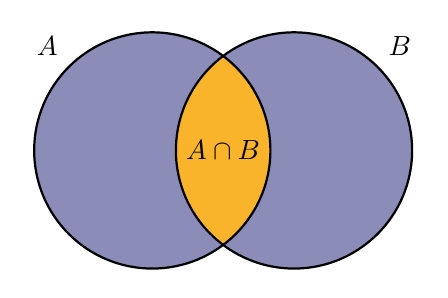
\begin{tikzpicture}[thick, set/.style = {circle, minimum size = 3cm, fill=MidnightBlue!50}]
		\node[set,label={135:$A$}] (A) at (0,0) {};
		\node[set,label={45:$B$}] (B) at (1.8,0) {};

		\begin{scope}
			\clip (0,0) circle(1.5cm);
			\clip (1.8,0) circle(1.5cm);
			\fill[Dandelion](0,0) circle(1.5cm);
		\end{scope}

		\draw (0,0) circle(1.5cm);
		\draw (1.8,0) circle(1.5cm);
		\node at (0.9,0) {$ A \cap B $};
	\end{tikzpicture}
	\caption{交集}
\end{figure}

如果两个集合没有公共元素,那么它们的交集为空集。

\subsection{并集(Union)}

假设$ A $和$ B $是两个集合,由它们所有元素合并在一起组成的集合,称为$ A $与$ B $的并集,表示为$ A \cup B $。

\begin{figure}[H]
	\centering
	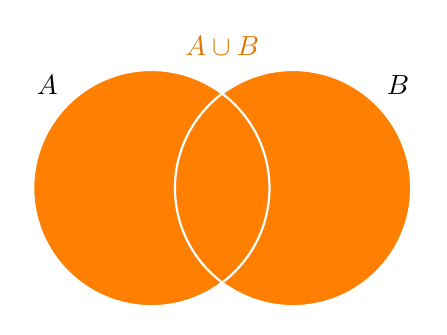
\begin{tikzpicture}
		\node [circle, fill=orange, minimum size=3cm, label={135:$A$}] (A) at (0,0){};
		\node [circle,
			fill=orange,
			minimum size =3cm,
			label={45:$B$}] (B) at (1.8,0){};

		\draw[white,thick] (0,0) circle(1.5cm);
		\draw[white,thick] (1.8,0) circle(1.5cm);
		\node[orange!90!black] at (0.9,1.8) {$ A \cup B $};
	\end{tikzpicture}
	\caption{并集}
\end{figure}

\subsection{差集(Difference)}

假设$ A $和$ B $是两个集合,由属于$ A $而不属于$ B $的元素组成的集合,称为$ A $与$ B $的差集,表示为$ A - B $。 \\

差集运算不满足交换律,即$ A - B \neq B - A $。

\begin{figure}[H]
	\centering
	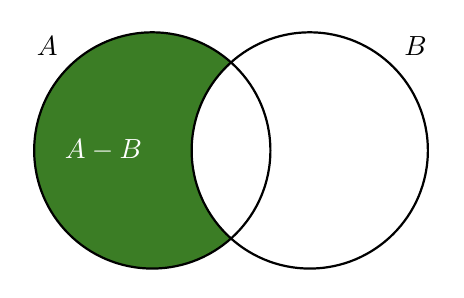
\begin{tikzpicture}[thick, set/.style = { circle, minimum size = 3cm}]
		\node[set,fill=OliveGreen,label={135:$A$}] (A) at (0,0) {};
		\node[set,fill=white,label={45:$B$}] (B) at (0:2) {};

		\draw (0,0) circle(1.5cm);
		\draw (2,0) circle(1.5cm);
		\node[left,white] at (A.center){$ A - B $};
	\end{tikzpicture}
	\caption{差集$ A - B $}
\end{figure}

\begin{figure}[H]
	\centering
	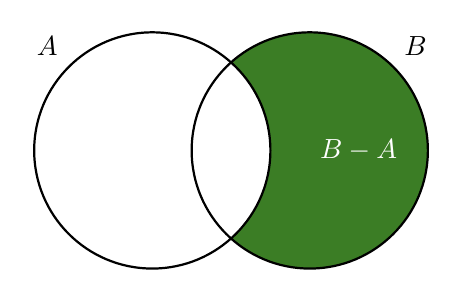
\begin{tikzpicture}[thick, set/.style = { circle, minimum size = 3cm}]
		\node[set,fill=OliveGreen,label={45:$B$}] (B) at (0:2) {};
		\node[set,fill=white,label={135:$A$}] (A) at (0,0) {};

		\draw (0,0) circle(1.5cm);
		\draw (2,0) circle(1.5cm);

		\node[right,white] at (B.center){$ B - A $};
	\end{tikzpicture}
	\caption{差集$ B - A $}
\end{figure}

\newpage

\section{集合恒等式}

\subsection{集合恒等式}

集合恒等式可以直接由对应的逻辑等价式证明。

\begin{tcolorbox}
	\mybox{幂等律 Idempotent Laws}
	\begin{align}
		A \cap A = A \\
		A \cup A = A
	\end{align}
\end{tcolorbox}

\begin{tcolorbox}
	\mybox{恒等律 Identity Laws}
	\begin{align}
		A \cap U = A \\
		A \cup \emptyset = A
	\end{align}
\end{tcolorbox}

\begin{tcolorbox}
	\mybox{支配律 Domination Laws}
	\begin{align}
		A \cap \emptyset = \emptyset \\
		A \cup U = U
	\end{align}
\end{tcolorbox}

\begin{tcolorbox}
	\mybox{双非律 Double Negation Law}
	\begin{align}
		\overline {\overline A} = A
	\end{align}
\end{tcolorbox}

\begin{tcolorbox}
	\mybox{交换律 Commutative Laws}
	\begin{align}
		A \cap B = B \cap A \\
		A \cup B = B \cup A
	\end{align}
\end{tcolorbox}

\begin{tcolorbox}
	\mybox{结合律 Associative Laws}
	\begin{align}
		(A \cap B) \cap C = A \cap (B \cap C) \\
		(A \cup B) \cup C = A \cup (B \cup C)
	\end{align}
\end{tcolorbox}

\begin{tcolorbox}
	\mybox{分配律 Distributive Laws}
	\begin{align}
		A \cap (B \cup C) = (A \cap B) \cup (A \cap C) \\
		A \cup (B \cap C) = (A \cup B) \cap (A \cup C)
	\end{align}
\end{tcolorbox}

\begin{tcolorbox}
	\mybox{德摩根律 De Morgan's Laws}
	\begin{align}
		\overline{A \cap B} = \overline A \cup \overline B
	\end{align}
\end{tcolorbox}

\begin{tcolorbox}
	\mybox{吸收律 Absorption Laws}
	\begin{align}
		A \cap (A \cup B) = A \\
		A \cup (A \cap B) = A
	\end{align}
\end{tcolorbox}

\begin{tcolorbox}\nonumber
	\mybox{证明}
	$ \overline{A \cup (B \cap C)} = (\overline C \cup \overline B) \cap \overline A $
	\begin{align}
		 & \overline{A \cup (B \cap C)}                      \\
		 & = \overline A \cap \overline{B \cap C}            \\
		 & = \overline A \cap (\overline B \cup \overline C) \\
		 & = (\overline B \cup \overline C) \cap \overline A \\
		 & = (\overline C \cup \overline B) \cap \overline A
	\end{align}
\end{tcolorbox}

\begin{tcolorbox}
	\mybox{Exercise}
	一共有40个学生,有3门课程可供学生选择(C语言、离散数学、软件工程)。 \\
	7人没有选任何课程; \\
	16人选软件工程; \\
	10人选C语言; \\
	5人同时选离散数学和软件工程; \\
	4人同时选离散数学和C语言; \\
	3人同时选软件工程和C语言; \\
	2人同时选离散数学、软件工程和C语言。 \\

	\begin{figure}[H]
		\centering
		\begin{tikzpicture}
			\tikzset{venn circle/.style={draw,circle,minimum width=6cm,fill=#1,opacity=0.4}}
			\node [] () at (-2, -3) {C语言};
			\node [] () at (2, 7) {离散数学};
			\node [] () at (6, -3) {软件工程};
			\node [] () at (6, 7) {$ U $};
			\node [] () at (6, 6.5) {7};
			\node [venn circle = red] (A) at (0,0) {5};
			\node [venn circle = blue] (B) at (60:4cm) {10};
			\node [venn circle = green] (C) at (0:4cm) {10};
			\node[left] at (barycentric cs:A=1/2,B=1/2) {2};
			\node[below] at (barycentric cs:A=1/2,C=1/2) {1};
			\node[right] at (barycentric cs:B=1/2,C=1/2) {3};
			\node[below] at (barycentric cs:A=1/3,B=1/3,C=1/3) {2};
		\end{tikzpicture}
	\end{figure}
\end{tcolorbox}

\newpage

\section{笛卡尔积}

\subsection{元组(Tuple)}

有时候元素聚集中次序是很重要的,由于集合是无序的,所以就需要一种不同的结构表示有序的聚集,这就是有序$ n $元组(ordered-n-tuple)。 \\

有序$ n $元组$ (a_1,\ a_2,\ \dots,\ a_n) $是以$ a_1 $为第$ 1 $个元素,$ a_2 $为第$ 2 $个元素,$ a_n $为第$ n $个元素的有序聚集。 \\

只有两个有序$ n $元组的每一对对应的元素都相等,那么这两个有序$ n $元组是相等的,即:

$$
	(a_1,\ a_2,\ \dots,\ a_n) = (b_1,\ b_2,\ \dots,\ b_n)\ \text{iff}\ i = 1,\ 2,\ \dots,\ n
$$

需要注意,$ (a,\ b) $与$ (b,\ a) $不相等,除非$ a = b $。

\subsection{笛卡尔积(Cartesian Product)}

假设有两个集合$ A $和$ B $,$ A $和$ B $的笛卡尔积用$ A \times B $表示,笛卡尔积是所有序偶$ (a,\ b) $的集合,其中$ a \in A $且$ b \in B $。

$$
	A \times B = \{(a,\ b)\ |\ a \in A \wedge b \in B\}
$$

笛卡尔积$ A \times B $和$ B \times A $是不相等的,除非$ A = \emptyset $或$ B = \emptyset $或$ A = B $。

\begin{tcolorbox}
	\mybox{Exercise}
	笛卡尔积 \\
	学生集合$ S = \{s1,\ s2\} $ \\
	课程集合$ C = \{c1,\ c2,\ c3\} $ \\
	$ S \times C = \{(s1,\ c1),\ (s1,\ c2),\ (s1,\ c3),\ (s2,\ c1),\ (s2,\ c2),\ (s2,\ c3)\} $ \\
	笛卡尔积$ S \times C $表示学生选课的所有可能情况 \\
\end{tcolorbox}

\begin{tcolorbox}\nonumber
	\mybox{Exercise}
	笛卡尔积$ A \times B \times C $ \\
	$ A = \{0,\ 1\} $ \\
	$ B = \{1,\ 2\} $ \\
	$ C = \{0,\ 1,\ 2\} $
	\begin{align}
		A \times B \times C = \{(0, 1, 0), (0, 1, 1), (0, 1, 2), (0, 2, 0), (0, 2, 1), (0, 2, 2), \\
		(1, 1, 0), (1, 1, 1), (1, 1, 2), (1, 2, 0), (1, 2, 1), (1, 2, 2)\}
	\end{align}
\end{tcolorbox}

一个集合与自身的笛卡尔积,如$ A \times A $可表示为$ A^2 $。

\begin{tcolorbox}
	\mybox{Exercise}
	笛卡尔积$ A^2 $ \\
	$ A = \{1,\ 2\} $ \\
	$ A^2 = \{(1,\ 1),\ (1,\ 2),\ (2,\ 1),\ (2,\ 2)\} $
\end{tcolorbox}

\newpage

\chapter{函数}

\section{函数}

\subsection{函数(Function)}

函数在数学和计算机科学中的概念非常重要,在离散数学中函数用于定义像序列和字符串这样的离散结构。 \\

利用一个函数$ f $,可以将一个值$ x \in \mathbb{R} $映射(mapping)到一个特定的值$ y = f(x),\ y \in \mathbb{R} $ 上。 \\

假设有两个非空集合$ X $和$ Y $,从$ X $到$ Y $的函数$ f $是指对于$ X $的每个元素恰好都对应$ Y $的一个元素,即$ f(x) = y,\ x \in X,\ y \in Y $,那么就写成$ f: X \rightarrow Y $。 \\

集合$ X $被称为函数$ f $的定义域(domain),集合$ Y $被称为函数$ f $的陪域(co-domain)。 \\

如果$ f(x) = y $,那么$ y $是$ x $在函数$ f $下的像(image),$ x $是$ y $在函数$ f $下的原像(pre-image)。函数$ f $的值域(range)是集合$ X $中所有像的集合。 \\

当两个函数$ f $和$ g $有相同的定义域和陪域,并且对于定义域中所有元素$ x $都满足$ f(x) = g(x) $,那么函数$ f $和$ g $相等,表示为$ f = g $。

\begin{tcolorbox}
	\mybox{Exercise}
	判断是否为函数 \\
	\begin{figure}[H]
		\centering
		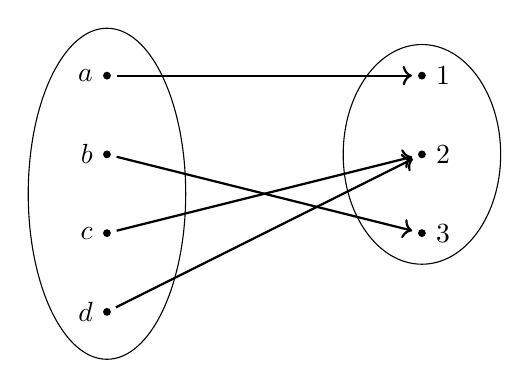
\begin{tikzpicture}[ele/.style={fill=black,circle,minimum width=.8pt,inner sep=1pt},every fit/.style={ellipse,draw,inner sep=-2pt}]
			\node[ele,label=left:$a$] (a) at (0,4) {};
			\node[ele,label=left:$b$] (b) at (0,3) {};
			\node[ele,label=left:$c$] (c) at (0,2) {};
			\node[ele,label=left:$d$] (d) at (0,1) {};

			\node[ele,,label=right:$1$] (v1) at (4,4) {};
			\node[ele,,label=right:$2$] (v2) at (4,3) {};
			\node[ele,,label=right:$3$] (v3) at (4,2) {};

			\node[draw,fit= (a) (b) (c) (d),minimum width=2cm] {} ;
			\node[draw,fit= (v1) (v2) (v3),minimum width=2cm] {} ;
			\draw[->,thick,shorten <=2pt,shorten >=2] (a) -- (v1);
			\draw[->,thick,shorten <=2pt,shorten >=2] (b) -- (v3);
			\draw[->,thick,shorten <=2pt,shorten >=2] (c) -- (v2);
			\draw[->,thick,shorten <=2pt,shorten >=2] (d) -- (v2);
		\end{tikzpicture}
		\caption{函数}
	\end{figure}

	\begin{figure}[H]
		\centering
		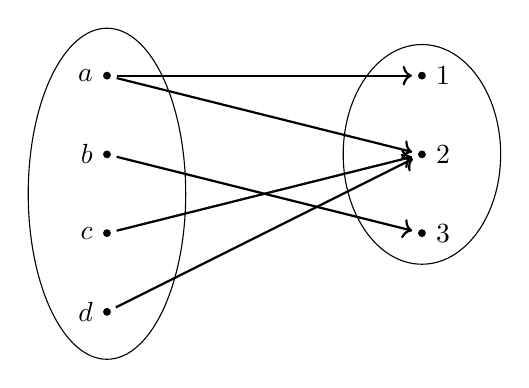
\begin{tikzpicture}[ele/.style={fill=black,circle,minimum width=.8pt,inner sep=1pt},every fit/.style={ellipse,draw,inner sep=-2pt}]
			\node[ele,label=left:$a$] (a) at (0,4) {};
			\node[ele,label=left:$b$] (b) at (0,3) {};
			\node[ele,label=left:$c$] (c) at (0,2) {};
			\node[ele,label=left:$d$] (d) at (0,1) {};

			\node[ele,,label=right:$1$] (v1) at (4,4) {};
			\node[ele,,label=right:$2$] (v2) at (4,3) {};
			\node[ele,,label=right:$3$] (v3) at (4,2) {};

			\node[draw,fit= (a) (b) (c) (d),minimum width=2cm] {} ;
			\node[draw,fit= (v1) (v2) (v3),minimum width=2cm] {} ;
			\draw[->,thick,shorten <=2pt,shorten >=2] (a) -- (v1);
			\draw[->,thick,shorten <=2pt,shorten >=2] (a) -- (v2);
			\draw[->,thick,shorten <=2pt,shorten >=2] (b) -- (v3);
			\draw[->,thick,shorten <=2pt,shorten >=2] (c) -- (v2);
			\draw[->,thick,shorten <=2pt,shorten >=2] (d) -- (v2);
		\end{tikzpicture}
		\caption{非函数}
	\end{figure}
\end{tcolorbox}

\begin{tcolorbox}
	\mybox{Exercise}
	\begin{figure}[H]
		\centering
		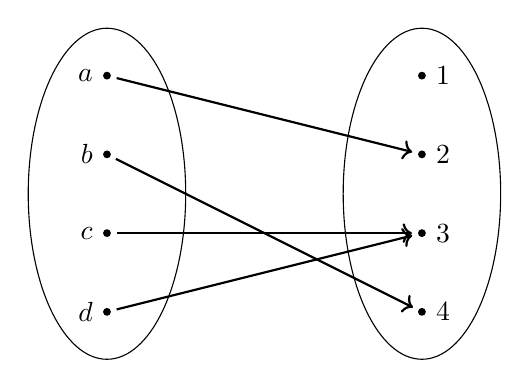
\begin{tikzpicture}[ele/.style={fill=black,circle,minimum width=.8pt,inner sep=1pt},every fit/.style={ellipse,draw,inner sep=-2pt}]
			\node[ele,label=left:$a$] (a) at (0,4) {};
			\node[ele,label=left:$b$] (b) at (0,3) {};
			\node[ele,label=left:$c$] (c) at (0,2) {};
			\node[ele,label=left:$d$] (d) at (0,1) {};

			\node[ele,,label=right:$1$] (v1) at (4,4) {};
			\node[ele,,label=right:$2$] (v2) at (4,3) {};
			\node[ele,,label=right:$3$] (v3) at (4,2) {};
			\node[ele,,label=right:$4$] (v4) at (4,1) {};

			\node[draw,fit= (a) (b) (c) (d),minimum width=2cm] {} ;
			\node[draw,fit= (v1) (v2) (v3) (v4),minimum width=2cm] {} ;
			\draw[->,thick,shorten <=2pt,shorten >=2] (a) -- (v2);
			\draw[->,thick,shorten <=2pt,shorten >=2] (b) -- (v4);
			\draw[->,thick,shorten <=2pt,shorten >=2] (c) -- (v3);
			\draw[->,thick,shorten <=2pt,shorten >=2] (d) -- (v3);
		\end{tikzpicture}
	\end{figure}

	是否为函数:是 \\
	定义域(domain):$ a,\ b,\ c,\ d $ \\
	陪域(co-domain):$ 1,\ 2,\ 3,\ 4 $ \\
	值域(range):$ 2,\ 3,\ 4 $
\end{tcolorbox}

\newpage

\section{取整函数}

\subsection{上取整函数(Ceiling Function)}

取整函数包括上取整和下取整,可以将实数映射到整数($ \mathbb{R} \rightarrow \mathbb{Z} $),它们以不同的方式将实数近似到相邻的整数。 \\

上取整函数将实数$ x $向上取到大于或等于$ x $的最小整数,表示为$ \lceil x \rceil $。

\begin{tcolorbox}
	\mybox{Exercise}
	上取整函数 \\
	$ \lceil 3.2 \rceil = 4 $ \\
	$ \lceil 2.6 \rceil = 3 $ \\
	$ \lceil -0.5 \rceil = 0 $
\end{tcolorbox}

\subsection{下取整函数(Floor Function)}

下取整函数将实数$ x $向下取到小于或等于$ x $的最大整数,表示为$ \lfloor x \rfloor $。

\begin{tcolorbox}
	\mybox{Exercise}
	下取整函数 \\
	$ \lfloor 3.2 \rfloor = 3 $ \\
	$ \lfloor 5.9 \rfloor = 5 $ \\
	$ \lfloor -0.5 \rfloor = -1 $
\end{tcolorbox}

\newpage

\section{函数分类}

\subsection{一对一函数(One-to-one) / 单射函数(Injection)}

一对一函数 / 单射函数是指对于函数$ f $的定义域中所有的$ a $和$ b $,如果$ a \neq b $,那么$ f(a) \neq f(b) $。

\begin{figure}[H]
	\centering
	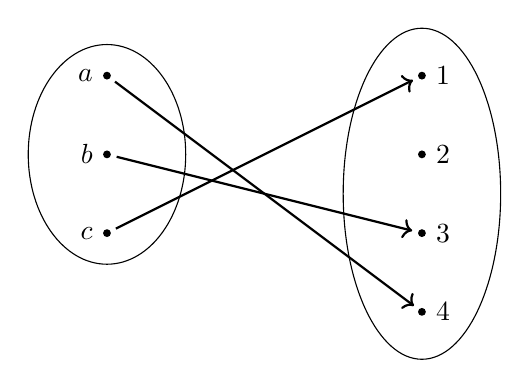
\begin{tikzpicture}[ele/.style={fill=black,circle,minimum width=.8pt,inner sep=1pt},every fit/.style={ellipse,draw,inner sep=-2pt}]
		\node[ele,label=left:$a$] (a) at (0,4) {};
		\node[ele,label=left:$b$] (b) at (0,3) {};
		\node[ele,label=left:$c$] (c) at (0,2) {};

		\node[ele,,label=right:$1$] (v1) at (4,4) {};
		\node[ele,,label=right:$2$] (v2) at (4,3) {};
		\node[ele,,label=right:$3$] (v3) at (4,2) {};
		\node[ele,,label=right:$4$] (v4) at (4,1) {};

		\node[draw,fit= (a) (b) (c),minimum width=2cm] {} ;
		\node[draw,fit= (v1) (v2) (v3) (v4),minimum width=2cm] {} ;
		\draw[->,thick,shorten <=2pt,shorten >=2] (a) -- (v4);
		\draw[->,thick,shorten <=2pt,shorten >=2] (b) -- (v3);
		\draw[->,thick,shorten <=2pt,shorten >=2] (c) -- (v1);
	\end{tikzpicture}
	\caption{一对一函数 / 单射函数}
\end{figure}

\begin{tcolorbox}
	\mybox{Exercise}
	一对一函数 / 单射函数 \\
	$ f(x) = x + 1 $是一对一函数。 \\
	$ f(x) = x^2 $不是一对一函数,因为$ f(1) = f(-1) = 1 $。
\end{tcolorbox}

\subsection{映上函数(Onto) / 满射函数(Surjection)}

映上函数 / 满射函数是指对于函数$ f: A \rightarrow B $,每个$ b \in B $都有元素$ a \in A $使得$ f(a) = b $。

\begin{figure}[H]
	\centering
	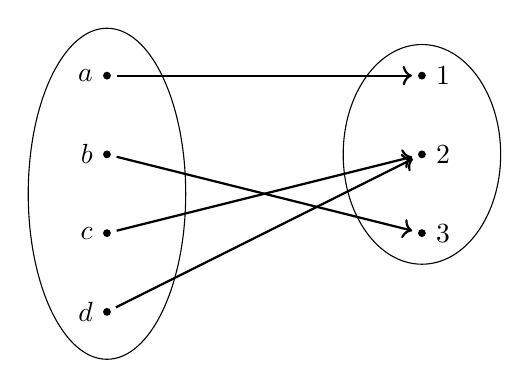
\begin{tikzpicture}[ele/.style={fill=black,circle,minimum width=.8pt,inner sep=1pt},every fit/.style={ellipse,draw,inner sep=-2pt}]
		\node[ele,label=left:$a$] (a) at (0,4) {};
		\node[ele,label=left:$b$] (b) at (0,3) {};
		\node[ele,label=left:$c$] (c) at (0,2) {};
		\node[ele,label=left:$d$] (d) at (0,1) {};

		\node[ele,,label=right:$1$] (v1) at (4,4) {};
		\node[ele,,label=right:$2$] (v2) at (4,3) {};
		\node[ele,,label=right:$3$] (v3) at (4,2) {};

		\node[draw,fit= (a) (b) (c) (d),minimum width=2cm] {} ;
		\node[draw,fit= (v1) (v2) (v3),minimum width=2cm] {} ;
		\draw[->,thick,shorten <=2pt,shorten >=2] (a) -- (v1);
		\draw[->,thick,shorten <=2pt,shorten >=2] (b) -- (v3);
		\draw[->,thick,shorten <=2pt,shorten >=2] (c) -- (v2);
		\draw[->,thick,shorten <=2pt,shorten >=2] (d) -- (v2);
	\end{tikzpicture}
	\caption{映上函数 / 满射函数}
\end{figure}

\begin{tcolorbox}
	\mybox{Exercise}
	映上函数 / 满射函数 \\
	$ f: \mathbb{Z} \rightarrow \mathbb{Z},\ f(x) = x + 1 $是映上函数。 \\
	$ f: \mathbb{Z} \rightarrow \mathbb{Z},\ f(x) = x^2 $不是映上函数,因为没有整数$ x $使$ x^2 = -1 $。
\end{tcolorbox}

\subsection{一一对应函数 / 双射函数(Bijection)}

如果一个函数既是一对一函数又是映上函数,那么这个函数就被称为一一对应函数 / 双射函数。

\begin{figure}[H]
	\centering
	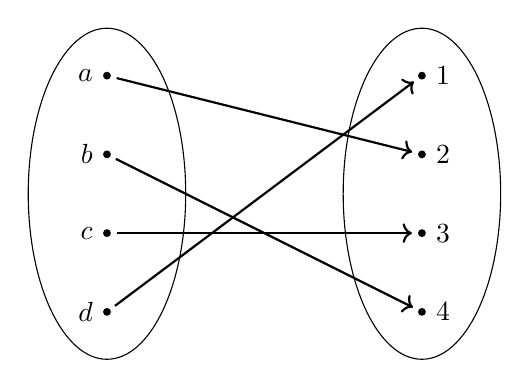
\begin{tikzpicture}[ele/.style={fill=black,circle,minimum width=.8pt,inner sep=1pt},every fit/.style={ellipse,draw,inner sep=-2pt}]
		\node[ele,label=left:$a$] (a) at (0,4) {};
		\node[ele,label=left:$b$] (b) at (0,3) {};
		\node[ele,label=left:$c$] (c) at (0,2) {};
		\node[ele,label=left:$d$] (d) at (0,1) {};

		\node[ele,,label=right:$1$] (v1) at (4,4) {};
		\node[ele,,label=right:$2$] (v2) at (4,3) {};
		\node[ele,,label=right:$3$] (v3) at (4,2) {};
		\node[ele,,label=right:$4$] (v4) at (4,1) {};

		\node[draw,fit= (a) (b) (c) (d),minimum width=2cm] {} ;
		\node[draw,fit= (v1) (v2) (v3) (v4),minimum width=2cm] {} ;
		\draw[->,thick,shorten <=2pt,shorten >=2] (a) -- (v2);
		\draw[->,thick,shorten <=2pt,shorten >=2] (b) -- (v4);
		\draw[->,thick,shorten <=2pt,shorten >=2] (c) -- (v3);
		\draw[->,thick,shorten <=2pt,shorten >=2] (d) -- (v1);
	\end{tikzpicture}
	\caption{一一对应函数 / 双射函数}
\end{figure}

\begin{tcolorbox}
	\mybox{Exercise}
	一一对应函数 / 双射函数 \\
	$ f $是从$ \{a,\ b,\ c,\ d\} $到$ \{1,\ 2,\ 3,\ 4\} $的函数,定义$ f(a) = 4,\ f(b) = 2,\ f(c) = 1,\ f(d) = 3 $。 \\
	函数$ f $是单射函数,因为没有两个值映射到相同的函数值。 \\
	函数$ f $是满射函数,因为陪域的个数与值域的个数相同。 \\
	因此,函数$ f $是双射函数。
\end{tcolorbox}

\newpage

\section{反函数}

\subsection{反函数(Inverse Function)}

假设有一个从集合$ A $到集合$ B $的双射函数$ f $。由于$ f $是满射函数,所以$ B $中的每个元素都是$ A $中某些元素的像;又由于$ f $还是单射函数,所以$ B $的每个元素都是$ A $中唯一一个元素的像。 \\

于是,通过把f的对应关系颠倒,获得的从$ B $到$ A $的新函数被称为$ f $的反函数,用$ f^{-1} $表示。当$ f(a) = b $时,$ f^{-1}(b) = a $。需要注意,不要将$ f^{-1} $与$ 1 \over f $混淆。

\begin{tcolorbox}
	\mybox{Exercise}
	反函数
	\begin{figure}[H]
		\centering
		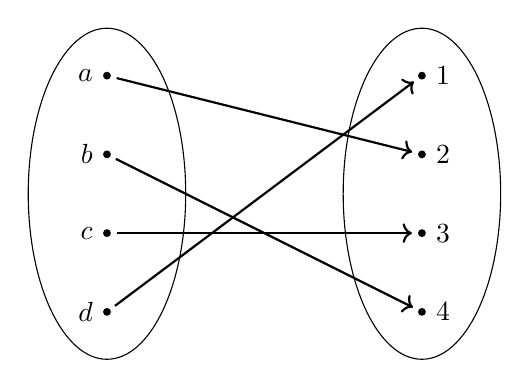
\begin{tikzpicture}[ele/.style={fill=black,circle,minimum width=.8pt,inner sep=1pt},every fit/.style={ellipse,draw,inner sep=-2pt}]
			\node[ele,label=left:$a$] (a) at (0,4) {};
			\node[ele,label=left:$b$] (b) at (0,3) {};
			\node[ele,label=left:$c$] (c) at (0,2) {};
			\node[ele,label=left:$d$] (d) at (0,1) {};

			\node[ele,,label=right:$1$] (v1) at (4,4) {};
			\node[ele,,label=right:$2$] (v2) at (4,3) {};
			\node[ele,,label=right:$3$] (v3) at (4,2) {};
			\node[ele,,label=right:$4$] (v4) at (4,1) {};

			\node[draw,fit= (a) (b) (c) (d),minimum width=2cm] {} ;
			\node[draw,fit= (v1) (v2) (v3) (v4),minimum width=2cm] {} ;
			\draw[->,thick,shorten <=2pt,shorten >=2] (a) -- (v2);
			\draw[->,thick,shorten <=2pt,shorten >=2] (b) -- (v4);
			\draw[->,thick,shorten <=2pt,shorten >=2] (c) -- (v3);
			\draw[->,thick,shorten <=2pt,shorten >=2] (d) -- (v1);
		\end{tikzpicture}
	\end{figure}
	是否有反函数:是 \\
	$ f^{-1}(2) = a $ \\
	$ f^{-1}(1) = 1 $
\end{tcolorbox}

\begin{tcolorbox}
	\mybox{Exercise}
	计算$ f(x) = x + 3 $的反函数 \\
	$ f^{-1}(x) = x - 3 $
\end{tcolorbox}

\newpage

\section{合成函数}

\subsection{合成函数(Composition Function)}

假设$ g $是从集合$ A $到集合$ B $的函数,$ f $是从集合$ B $到集合$ C $的函数。函数$ f $和$ g $的合成,记作$ f \circ g $。

$$
	(f \circ g)(x) = f(g(x))
$$

函数合成的顺序很重要,$ f \circ g $与$ g \circ f $并不相等。

\begin{tcolorbox}
	\mybox{Exercise}
	合成函数 \\
	$ f: \mathbb{R^+} \rightarrow \mathbb{R^+},\ f(x) = x^3 $ \\
	$ g: \mathbb{R^+} \rightarrow \mathbb{R^+},\ g(x) = x + 2 $ \\
	$ (f \circ g)(x) = f(g(x)) = (x + 2)^3 $ \\
	$ (g \circ f)(x) = g(f(x)) = x^3 + 2 $
\end{tcolorbox}

\subsection{恒等函数(Identity Function)}

如果一个从集合$ A $到集合$ B $的函数$ f $有反函数,那么$ f $与$ f^{-1} $的合成函数得到的是恒等函数。 \\

如果$ f(a) = b $,那么$ f^{-1}(b) = a $。

$$
	(f \circ f^{-1})(a) = f^{-1}(f(a)) = f^{-1}(b) = a
$$

\newpage

\section{指数函数与对数函数}

\subsection{指数函数(Exponential Function)}

指数函数的定义为$ y = a^x\ (a > 0\ |\ a \neq 1) $,其中$ a $称为底数(base),$ x $称为指数(exponent)。

\begin{figure}[H]
	\centering
	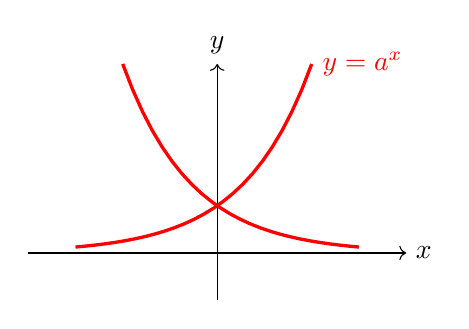
\begin{tikzpicture}[scale=0.6]
		\draw[->] (-4,0) -- (4,0) node[right] {$ x $};
		\draw[->] (0,-1) -- (0,4) node[above] {$ y $};
		\draw[very thick,color=red,domain=-3:2] plot (\x,{2 ^ \x}) node[right] {$ y = {a^x} $};
		\draw[very thick,color=red,domain=-2:3] plot (\x,{0.5 ^ \x});
	\end{tikzpicture}
	\caption{指数函数}
\end{figure}

\begin{tcolorbox}
	\mybox{指数函数}
	\begin{align}
		 & a^{-x} = {1 \over a^x}                    \\
		 & {1 \over a^{-x}} = a^x                    \\
		 & (ab)^x = a^xb^x                           \\
		 & ({a \over b})^x = {a^x \over b^x}         \\
		 & a^{kx} = (a^k)^x = (a^x)^k                \\
		 & a^ma^n = a^{m+n}                          \\
		 & {a^m \over a^n} = a^{m-n}                 \\
		 & a^{1/n} = \sqrt[n]{a}                     \\
		 & a^{m/n} = \sqrt[n]{a^m} = (\sqrt[n]{a})^m
	\end{align}
\end{tcolorbox}

\begin{tcolorbox}
	\mybox{Exercise}
	指数函数 \\
	$ (6^{2k})^3 = 6^{6k} $ \\
	$ 6^{k^2} \times 6 = 6^{k^2 + 1} $ \\
	$ {3^k \over 9} = {3^k \over 3^2} = 3^{k-2} $ \\
	$ 3^k \times 27 = 3^k \times 3^3 = 3^{k+3} $
\end{tcolorbox}

\subsection{对数函数(Logarithm Function)}

对于函数$ f: \{1,\ 2,\ 3,\ 4\} \rightarrow \{1,\ 4,\ 8,\ 16\},\ f(x) = 2^x $,指数函数是双射函数,因此它是有反函数的。 \\

对数函数是指数函数的反函数,对数函数的定义为$ y = log_a{x}\ (a > 0\ |\ a \neq 1) $,其中$ a $称为底数。

\begin{figure}[H]
	\centering
	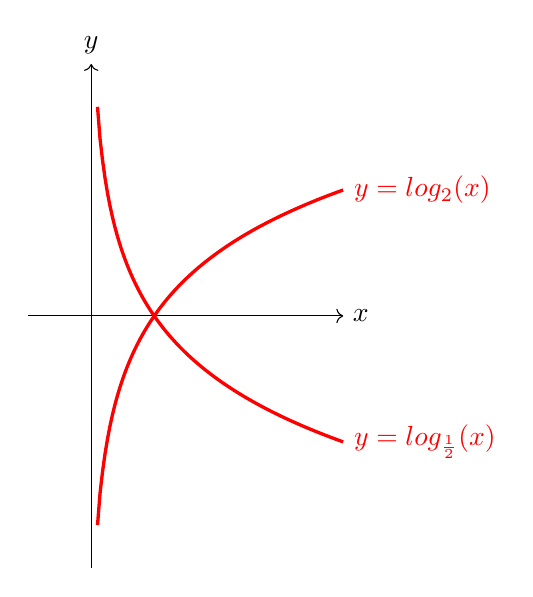
\begin{tikzpicture}[scale=0.8]
		\draw[->] (-1,0) -- (4,0) node[right] {$ x $};
		\draw[->] (0,-4) -- (0,4) node[above] {$ y $};
		\draw [very thick,color=red,domain=0.1:4,samples=100] plot (\x,{log2(\x)}) node[right] {$ y = log_2(x) $};
		\draw [very thick,color=red,domain=0.1:4,samples=100] plot (\x,{log10(\x) / log10(0.5)}) node[right] {$ y = log_{1 \over 2}(x) $};
	\end{tikzpicture}
	\caption{对数函数}
\end{figure}

\begin{tcolorbox}
	\mybox{对数函数}
	\begin{align}
		 & log_a(a^x) = x                                      \\
		 & a^{log_a(x)} = x                                    \\
		 & log_a(xy) = log_a(x) + log_a(y)                     \\
		 & log_a\left({x \over y}\right) = log_a(x) - log_a(y) \\
		 & log_a(x^n) = nlog_a(x)                              \\
		 & log_a(x) = {log_b(x) \over log_b(a)}
	\end{align}
\end{tcolorbox}

\begin{tcolorbox}
	\mybox{Exercise}
	对数函数 \\
	$ log_5{k} + log_5{2} = log_5{2k} $ \\
	$ log_2{5^2} = 2 \times log_2{5} $ \\
	$ {log_3{k^2} \over log_3{25}} = {2 \times log_3{k} \over log_3{5^2}} = {2 \times log_3{k} \over 2 \times log_3{5}} = log_5{k} $
\end{tcolorbox}

\newpage

\chapter{数论}

\section{进制转换}

\subsection{进制}

日常生活中都用十进制(decimal)来表示整数,十进制数由$ 0,\ 1,\ 2,\ 3,\ 4,\ 5,\ 6,\ 7,\ 8,\ 9 $这10个字符组成。一个十进制整数的第$ k $位的值可以由$ 10^{k-1} $计算得到。

\begin{tcolorbox}\nonumber
	\mybox{Exercise}
	十进制
	\begin{align}
		256 & = 200 + 50 + 6                                  \\
		    & = 2 \times 10^2 + 5 \times 10^1 + 6 \times 10^0
	\end{align}
\end{tcolorbox}

二进制(binary)、八进制(octal)、十六进制(hexadecimal)也是非常常用的表示法,例如计算机通常用二进制来做算术运算,而用八进制或十六进制来表示字符。

\subsection{进制转换}

一个$ b $进制的正整数$ n $可以唯一地构造展开式:

$$
	n = a^k \times b^k + a_{k-1} \times b^{k-1} + \dots + a_1 \times b^1 + a_0 \times b^0
$$

\begin{tcolorbox}
	\mybox{Exercise}
	$ b $进制转十进制 \\
	$ (1011)_2 = 1 \times 2^3 + 0 \times 2^2 + 1 \times 2^1 + 1 \times 2^0 = (11)_{10} $ \\
	$ (21022)_3 = 2 \times 3^4 + 1 \times 3^3 + 0 \times 3^2 + 2 \times 3^1 + 2 \times 3^0 = (197)_{10} $
\end{tcolorbox}

\begin{table}[H]
	\centering
	\setlength{\tabcolsep}{5mm}{
		\begin{tabular}{|c|c|c|c|}
			\hline
			\textbf{十进制} & \textbf{二进制} & \textbf{八进制} & \textbf{十六进制} \\
			\hline
			0               & 0               & 0               & 0                 \\
			\hline
			1               & 1               & 1               & 1                 \\
			\hline
			2               & 10              & 2               & 2                 \\
			\hline
			3               & 11              & 3               & 3                 \\
			\hline
			4               & 100             & 4               & 4                 \\
			\hline
			5               & 101             & 5               & 5                 \\
			\hline
			6               & 110             & 6               & 6                 \\
			\hline
			7               & 111             & 7               & 7                 \\
			\hline
			8               & 1000            & 10              & 8                 \\
			\hline
			9               & 1001            & 11              & 9                 \\
			\hline
			10              & 1010            & 12              & A                 \\
			\hline
			11              & 1011            & 13              & B                 \\
			\hline
			12              & 1100            & 14              & C                 \\
			\hline
			13              & 1101            & 15              & D                 \\
			\hline
			14              & 1110            & 16              & E                 \\
			\hline
			15              & 1111            & 17              & F                 \\
			\hline
		\end{tabular}
	}
	\caption{进制转换}
\end{table}

十进制转$ b $进制还可以使用短除法的方式。

\begin{tcolorbox}
	\mybox{Exercise}
	十进制转四进制 \\
	\begin{tabular}{rl}
		4\mydiv{637} & remainder 1 \\
		4\mydiv{159} & remainder 3 \\
		4\mydiv{39}  & remainder 3 \\
		4\mydiv{9}   & remainder 1 \\
		4\mydiv{2}   & remainder 2
	\end{tabular}
	$ (637)_{10} = (21331)_4 $
\end{tcolorbox}

\begin{tcolorbox}
	\mybox{Exercise}
	十进制转二进制 \\
	\begin{tabular}{rl}
		2\mydiv{637} & remainder 1 \\
		2\mydiv{318} & remainder 0 \\
		2\mydiv{159} & remainder 1 \\
		2\mydiv{79}  & remainder 1 \\
		2\mydiv{39}  & remainder 1 \\
		2\mydiv{19}  & remainder 1 \\
		2\mydiv{9}   & remainder 1 \\
		2\mydiv{4}   & remainder 0 \\
		2\mydiv{2}   & remainder 0 \\
		2\mydiv{1}   & remainder 1
	\end{tabular}
	$ (637)_{10} = (1001111101)_2 $
\end{tcolorbox}

\begin{tcolorbox}
	\mybox{Exercise}
	十进制转八进制 \\
	\begin{tabular}{rl}
		8\mydiv{1000} & remainder 0 \\
		8\mydiv{125}  & remainder 5 \\
		8\mydiv{15}   & remainder 7 \\
		8\mydiv{1}    & remainder 1
	\end{tabular}
	$ (1000)_{10} = (1750)_8 $
\end{tcolorbox}

\newpage

\section{素数}

\subsection{素数(Prime Numbers)}

基于整除性的一个重要概念就是素数,素数是大于1的且不能被1和它自身以外的正整数整除的整数。素数是现代密码学中必不可少的一部分,密码学中的大素数就用在信息加密的某些方法中。

\begin{tcolorbox}
	\mybox{Exercise}
	判断素数 \\
	7是素数,因子有1和7。 \\
	9是合数,因为9能被3整除。
\end{tcolorbox}

每个大于1的整数都可以唯一地写成多个素数的乘积。

\begin{tcolorbox}
	\mybox{Exercise}
	素因子分解 \\
	$ 100 = 2 \times 2 \times 5 \times 5 = 2^2 \times 5^2 $ \\
	$ 999 = 3 \times 3 \times 3 \times 37 = 3^3 \times 37 $ \\
	$ 1024 = 2^{10} $
\end{tcolorbox}

如果$ n $是一个合数,那么$ n $必有一个素因子小于或等于$ \sqrt{n} $。

\begin{tcolorbox}
	\mybox{Exercise}
	证明101是素数 \\
	不超过$ \sqrt{101} $的素数只有$ 2, 3, 5, 7 $,因为$ 101 $不能被$ 2, 3, 5, 7 $整除,所以$ 101 $是素数。
\end{tcolorbox}

\vspace{-0.5cm}
\begin{lstlisting}[language=Python]
import math

def is_prime(num):
	for i in range(2, int(math.sqrt(num)) + 1):
		if num % i == 0:
			return False
	return True

def main():
	print(is_prime(13))
	print(is_prime(18))

if __name__ == "__main__":
	main()
\end{lstlisting}

埃拉托斯特尼筛法(Sieve of Eratosthenes)可以用来寻找不超过一个给定整数的所有素数。 \\

步骤:

\begin{enumerate}
	\item 建立包含所有给定整数以内的表格
	\item 从$ i = 2 $开始
	\item 移除所有整数$ n \% i == 0 $(除$ i $以外)
	\item $ i = i + 1 $
	\item 重复第3步和第4步
\end{enumerate}

\begin{table}[H]
	\centering
	\setlength{\tabcolsep}{5mm}{
		\begin{tabular}{|c|c|c|c|c|c|c|c|c|c|}
			\hline
			   & 2  & 3  & 4  & 5  & 6  & 7  & 8  & 9  & 10 \\
			\hline
			11 & 12 & 13 & 14 & 15 & 16 & 17 & 18 & 19 & 20 \\
			\hline
			21 & 22 & 23 & 24 & 25 & 26 & 27 & 28 & 29 & 30 \\
			\hline
		\end{tabular}
	}
	\caption{埃拉托斯特尼筛法}
\end{table}

\newpage

\section{序列}

\subsection{序列(Sequence)}

序列是一种用来表示有序列表的离散结构。例如$ 1,\ 2,\ 3,\ 5,\ 8 $是一个含有五项的序列,而$ 1,\ 3,\ 9,\ 27,\ 81,\ \dots $是一个无穷序列。序列可以用记号$ \{a_n\} $表示。

\begin{itemize}
	\item 递增序列(increasing sequence): 一个序列任意相邻的两项满足$ a_k < a_{k+1} $
	\item 非递减序列(non-decreasing sequence): 一个序列任意相邻的两项满足$ a_k \le a_{k+1} $
	\item 递减序列(decreasing sequence): 一个序列任意相邻的两项满足$ a_k > a_{k+1} $
	\item 非递增序列(non-increasing sequence): 一个序列任意相邻的两项满足$ a_k \ge a_{k+1} $
\end{itemize}

\begin{tcolorbox}
	\mybox{Exercise}
	序列 \\
	$ \{a_n\},\ a_n = {1 \over n}:\ 1,\ {1 \over 2},\ {1 \over 3},\ {1 \over 4},\ \dots $ \\
	$ \{b_n\},\ b_n = 2^n:\ 1,\ 2,\ 4,\ 8,\ 16,\ 32,\ \dots $
\end{tcolorbox}

\subsection{算术级数(Arithmetic Sequence)}

算术级数也称等差级数,序列形式如下:

$$
	a,\ a + d,\ a + 2d,\ \dots,\ a + nd,\ \dots\ (a, d \in \mathbb{R})
$$

\begin{tcolorbox}
	\mybox{Exercise}
	算术级数 \\
	$ \{a_n\},\ a_n = -1 + 4n:\ -1,\ 3,\ 7,\ 11,\ \dots $ \\
	$ \{b_n\},\ b_n = 7 - 3n:\ 7,\ 4,\ 1,\ -2,\ \dots $
\end{tcolorbox}

\subsection{几何级数(Geometric Sequence)}

几何级数也称等比级数,序列形式如下:

$$
	a,\ ar,\ ar^2,\ \dots,\ ar^n,\ \dots,\ (a, r \in \mathbb{R})
$$

\begin{tcolorbox}
	\mybox{Exercise}
	几何级数 \\
	$ \{a_n\},\ a_n = (-1)^n:\ 1,\ -1,\ 1,\ -1,\ 1,\ \dots $ \\
	$ \{b_n\},\ b_n = -2 \times 5^n:\ 2,\ 10,\ 50,\ 250,\ 1250,\ \dots $ \\
	$ \{c_n\},\ c_n = 6 \times ({1 \over 3})^n:\ 6,\ 2,\ {2 \over 3},\ {2 \over 9},\ {2 \over 27},\ \dots $
\end{tcolorbox}

\newpage

\section{递推关系}

\subsection{递推(Recurrence)}

如果数列$ \{a_n\} $的第$ n $项与它前一项的关系可以用一个公式来表示,那么这个公式就叫做这个数列的递推方程。 \\

算术级数的递推关系:

\vspace{-1cm}
\begin{align}
	\nonumber
	a_0 & = a           \\
	\nonumber
	a_n & = a_{n-1} + d
\end{align}

几何级数的递推关系:

\vspace{-1cm}
\begin{align}
	\nonumber
	a_0 & = a                \\
	\nonumber
	a_n & = a_{n-1} \times r
\end{align}

\begin{tcolorbox}\nonumber
	\mybox{Exercise}
	银行储蓄账户上有10000元,年利率为5.8\%,7年后账户中将有多少钱?
	\begin{align}
		P_n & = P_{n-1} + 0.058P_{n-1}                      \\
		    & = (1.058)P_{n-1}                              \\
		\\
		P_0 & = 10000                                       \\
		P_1 & = (1.058)P_0                                  \\
		P_2 & = (1.058)P_1 = (1.058)^2 P_0                  \\
		\dots                                               \\
		P_7 & = (1.058)P_6 = (1.058)^7 P_0 \approx 14838.83
	\end{align}
\end{tcolorbox}

\subsection{斐波那契数列(Fibonacci Sequence)}

斐波那契数列$ f_0,\ f_1,\ f_2,\ \dots $的递推公式为:

\begin{align}\nonumber
	f(n) = \begin{cases}
		1               & n = 1 \\
		1               & n = 2 \\
		f(n-1) + f(n-2) & n > 3
	\end{cases}
\end{align}

斐波那契数列的通项公式为:

$$
	f_n = {1 \over \sqrt{5}} \left({1 + \sqrt{5} \over 2} \right)^{n+1} - {1 \over \sqrt{5}} \left({1 - \sqrt{5} \over 2} \right)^{n+1}
$$

\begin{lstlisting}[language=C, title=斐波那契数列(递归)]
int fibonacci(int n) {
	if(n == 1 || n == 2) {
		return 1;
	}
	return fibonacci(n-2) + fibonacci(n-1);
}
\end{lstlisting}

\begin{figure}[H]
	\centering
	\begin{tikzpicture}[
			level distance=2cm,
			level 1/.style={sibling distance=6cm},
			level 2/.style={sibling distance=3cm},
			level 3/.style={sibling distance=2cm}
		]
		\node {$ f(5) $}
		child {
				node {$ f(3) $}
				child {node {$ f(1) $}}
				child {
						node {$ f(2) $}
						child {node {$ f(0) $}}
						child {node {$ f(1) $}}
					}
			}
		child {
				node {$ f(4) $}
				child {
						node {$ f(2) $}
						child {node {$ f(0) $}}
						child {node {$ f(1) $}}
					}
				child {
						node {$ f(3) $}
						child {node {$ f(1) $}}
						child {
								node {$ f(2) $}
								child {node {$ f(0) $}}
								child {node {$ f(1) $}}
							}
					}
			};
	\end{tikzpicture}
	\caption{递归树}
\end{figure}

\begin{lstlisting}[language=C, title=斐波那契数列(迭代)]
int fibonacci(int n) {
	int f[n];
	f[0] = f[1] = 1;
	for(int i = 2; i < n; i++) {
		f[i] = f[i-2] + f[i-1];
	}
	return f[n-1];
}
\end{lstlisting}

\newpage

\section{求和}

\subsection{求和(Summation)}

求和符号$ \sum $可以用于表示序列中所有项的累加和。

$$
	\sum_{i=lower}^{upper} a_i
$$

\begin{tcolorbox}
	\mybox{Exercise}
	求和 \\
	$ \sum_{i=1}^{100} i = 1 + 2 +3 + \dots + 99 + 100 = 5050 $ \\
	$ \sum_{j=1}^{5} j^2 = 1^2 + 2^2 + 3^2 + 4^2 + 5^2 = 55 $ \\
	$ \sum_{k=4}^{6} (-1)^k = (-1)^4 + (-1)^5 + (-1)^6 = 1 - 1 + 1 = 1 $
\end{tcolorbox}

\subsection{双重求和}

很多情况下需要使用双重求和,比如在计算机程序中嵌套循环的分析中。 \\

计算双重求和的方法是先展开内层求和,再继续计算外层求和。

\begin{tcolorbox}\nonumber
	\mybox{Exercise}
	双重求和
	\begin{align}
		 & \sum_{i=1}^{4} \sum_{j=1}^{3} ij \\
		 & = \sum_{i=1}^{4} (i + 2i + 3i)   \\
		 & = \sum_{i=1}^{4} 6i              \\
		 & = 6 + 12 + 1 8 + 24              \\
		 & = 60
	\end{align}
\end{tcolorbox}

\newpage

\section{数学归纳法}

\subsection{数学归纳法(Mathematical Induction)}

数学归纳法是一种数学证明方法,通常被用于证明某个给定命题在一个给定范围内成立。 \\

数学归纳法分为三个步骤:

\begin{enumerate}
	\item 归纳基础
	\item 归纳假设
	\item 归纳递推
\end{enumerate}

\begin{tcolorbox}\nonumber
	\mybox{证明}
	$ \sum_{i=1}^{n} i = {n(n+1) \over 2},\ n \in \mathbb{Z^+} $
	\begin{enumerate}
		\item 归纳基础:当$ n = 1 $,\\
		      $ \sum_{i=1}^{1} i = {1(1+1) \over 2} = 1 $

		\item 归纳假设:假设$ n = k $, \\
		      $ \sum_{i=1}^{k} i = {k(k+1) \over 2} $成立

		\item 归纳递推:证明$ n = k + 1 $时,
		      \begin{align}
			      \sum_{i=1}^{k+1} i & = \sum_{i=1}^{k} i + k + 1  \\
			                         & = {k(k+1) \over 2} + k + 1  \\
			                         & = {k(k+1) + 2(k+1) \over 2} \\
			                         & = {(k+1)(k+2) \over 2}
		      \end{align}
	\end{enumerate}
\end{tcolorbox}

\begin{tcolorbox}\nonumber
	\mybox{证明}
	$ 2^n \ge 3n,\ n \ge 4 $
	\begin{enumerate}
		\item 归纳基础:当$ n = 4 $,\\
		      $ 2^4 \ge 3 \times 4 $

		\item 归纳假设:假设$ n = k (n > 4) $, \\
		      $ 2^k \ge 3k $成立

		\item 归纳递推:证明$ n = k + 1 $时,
		      \begin{align}
			      2^{k+1} & = 2 \times 2^k  \\
			              & \ge 2 \times 3k \\
			              & = 3k + 3k       \\
			              & \ge 3k + 3      \\
			              & \ge 3(k+1)
		      \end{align}
	\end{enumerate}
\end{tcolorbox}

\newpage

\chapter{计数原理}

\section{计数原理}

\subsection{分类加法计数原理}

完成一件事有$ n $种不同的方案,其中第$ 1 $种方案有$ m_1 $种不同方法,第$ 2 $种方案有$ m_2 $种不同方法,$ \dots $,第$ n $种方案有$ m_n $种不同方法,那么完成这件事共有$ m_1 + m_2 + \dots + m_n $种不同方法。

\begin{tcolorbox}
	\mybox{Exercise}
	从A地到B地,可以乘火车、汽车、飞机。火车有4班、汽车2班、飞机3班,那么一天中乘坐这些交通工具从A地到B地有多少种不同的走法?
	$$
		4 + 2 + 3 = 9
	$$
\end{tcolorbox}

\subsection{分步乘法计数原理}

完成一件事需要$ n $个步骤,其中第$ 1 $个步骤有$ m_1 $种不同方法,第$ 2 $个步骤有$ m_2 $种不同方法,$ \dots $,第$ n $个步骤有$ m_n $种不同方法,那么完成这件事共有$ m_1 \times m_2 \times \dots m_n $种不同方法。

\begin{tcolorbox}
	\mybox{Exercise}
	一个书架的第1层有4本不同的计算机书,第2层有3本不同的经济书,第3层有2本不同的数学书。从书架的每一层各取一本书,有多少种不同取法?
	$$
		4 \times 3 \times 2 = 24
	$$
\end{tcolorbox}

\newpage

\section{排列}

\subsection{排列(Permutation)}

从$ n $个不同元素中取出$ m\ (m \le n) $ 个元素,按照一定次序排成一列,称为从$ n $个不同元素中取出$ m $个元素的一个排列。

\vspace{-1cm}
\begin{align}
	P_n^m = {n! \over (n-m)!}
\end{align}

例如一共有8个人,A、B、C、D、E、F、G、H。现在有3个奖杯,分别为金牌、银牌和铜牌。将这3个奖牌颁发给8个人中的3个,问颁发奖牌的不同方式总共有几种? \\

很明显这是一个排列的问题,因为把金牌先颁给A,再把银牌颁给B,跟把金牌先颁给B,再把银牌颁给A 这是两种不同的颁奖方式。

\begin{itemize}
	\item 第一步颁发金牌,金牌可以颁发给8个人中的1个,共有8种选择。

	\item 第二步颁发银牌,银牌可以颁发剩下7个人中的1个,共有7种选择。

	\item 第二步颁发铜牌,铜牌可以颁发剩下6个人中的1个,共有6种选择。
\end{itemize}

那么总共的颁奖方式共有$ 8 \times 7 \times 6 = 336 $种。

\begin{tcolorbox}
	\mybox{Exercise}
	用0-9这10个数字可以组成多少个没有重复数字的三位数? \\

	\textbf{方法一} \\
	由于0没有排在百位上,那么百位只能是1-9这9个数字任选1个,有$ P_9^1 $种选法。 \\
	对于十位和个位,从余下的9个数字种选2个,有$ P_9^2 $种选法。
	$$
		P_9^1 \times P_9^2 = 9 \times 9 \times 8 = 648
	$$

	\textbf{方法二} \\
	符合条件的三位数可以分为3大类:
	\begin{enumerate}
		\item 每一位数字都不是0的三位数,也就是从1-9中选3个,有$ P_9^3 $种选法。

		\item 个位数字为0,那么需要从剩下9个数字中选2个作为十位和百位,有$ P_9^2 $种选法。

		\item 十位数字为0,那么需要从剩下9个数字中选2个作为个位和百位,有$ P_9^2 $种选法。
	\end{enumerate}
	$$
		P_9^3 + P_9^2 + P_9^2 = 648
	$$

	\textbf{方法三} \\
	利用容斥法。从0-9这10个数字任取3个数字的排列数为$ P_{10}^3 $,其中0在百位上(也就是从1-9中选2个作为十位和个位)的排列数是$ P_9^2 $。
	$$
		P_{10}^3 - P_9^2 = 648
	$$
\end{tcolorbox}

\begin{tcolorbox}
	\mybox{Exercise}
	打印字符串math的全排列。
\end{tcolorbox}

\begin{lstlisting}[language=C, title=全排列]
#include <stdio.h>
#include <string.h>

void swap(char *a, char *b) {
	char temp = *a;
	*a = *b;
	*b = temp;
}

void permutation(char *s, int start, int end) {
	if(start >= end) {
		printf("%s\n", s);
	} else {
		for(int i = start; i < end; i++) {
			swap(s + i, s + start);
			permutation(s, start + 1, end);
			swap(s + i, s + start);
		}
	}
}

int main() {
	char s[] = "math";
	int len = strlen(s);
	permutation(s, 0, len);
	return 0;
}
\end{lstlisting}

\newpage

\section{组合}

\subsection{组合(Combination)}

从$ n $个不同元素中取出$ m\ (m \le n) $ 个元素,称为从$ n $个不同元素中取出$ m $个元素的一个组合。 \\

排列与组合的不同点在于,排列与元素的顺序有关,组合与元素的顺序无关。

\vspace{-1cm}
\begin{align}
	C_n^m = {P_n^m \over P_m^m} = {n! \over (n-m)!m!}
\end{align}

\begin{tcolorbox}
	\mybox{Exercise}
	在100件产品中,有98件合格品,2件次品,从这100件产品中任意抽出3件。 \\
	(1) 有多少种不同的抽法?
	$$
		C_{100}^3 = {100 \times 99 \times 98 \over 3 \times 2 \times 1} = 161700
	$$

	(2) 抽出的3件中恰好有1件事次品的抽法有多少种? \\
	2件次品抽出1件有$ C_2^1 $种,再从98件合格品种抽出2件合格品有$ C_{98}^2 $种。
	$$
		C_2^1 \times C_{98}^2 = 9506
	$$

	(3) 抽出的3件中至少有1件事次品的抽法有多少种? \\
	\textbf{方法一} \\
	恰好有1件次品有$ C_2^1 \times C_{98}^2 $种,恰好有2件次品有$ C_2^2 \times C_{98}^1 $种。
	$$
		C_2^1 \times C_{98}^2 + C_2^2 \times C_{98}^1 = 9604
	$$

	\textbf{方法二} \\
	利用容斥法。先从100件抽出3件有$ C_{100}^3 $种,其中3件都是合格品有$ C_{98}^3 $种。
	$$
		C_{100}^3 - C_{98}^3 = 9604
	$$
\end{tcolorbox}

\newpage

\section{古典概型}

\subsection{古典概型}

如果一个随机试验所包含的单位事件是有限的,且每个单位事件发生的可能性均相等,则这个随机试验叫做拉普拉斯试验,这种条件下的概率模型就叫古典概型。古典概型是概率论中最直观和最简单的模型,概率的许多运算规则,也首先是在这种模型下得到的。 \\

单位事件的特点是两两互斥的,例如抛一枚质地均匀的硬币时,正面朝上和背面朝上不会同时出现。 \\

在古典概型中,概率的计算公式为:

$$
	P(A) = {A\text{包含的单位事件个数}m \over \text{单位事件的总数}n}
$$

\begin{tcolorbox}
	\mybox{Exercise}
	掷两个质地均匀的骰子。 \\
	(1) 一共有多少种不同的结果?
	$$
		6 \times 6 = 36
	$$

	(2) 点数之和为9的结果有多少种? \\
	一共有4种:$ (3, 6), (6, 3), (4, 5), (5, 4) $ \\

	(3) 点数之和为9的概率是多少?
	$$
		P(A) = {4 \over 36} = {1 \over 9}
	$$
\end{tcolorbox}

\end{document}